\pdfoutput=1
\documentclass[aps,prd, amsmath,amssymb,superscriptaddress,showkeys,nofootinbib,reprint,preprintnumbers]{revtex4-1}
\usepackage{color}
\usepackage{aas_macros}
\usepackage{hyperref,breakurl}
\usepackage[usenames,dvipsnames]{xcolor}
\usepackage{dcolumn}
\usepackage{bm}
\usepackage{hyperref}
\usepackage{array}
\usepackage{dcolumn}

\usepackage{amsmath,amssymb,latexsym,times}
\DeclareMathOperator\arctanh{arctanh}

\usepackage{todonotes}
\newcommand{\verify}[1]{\textcolor{red}{\textbf{{#1}}}}

\newcommand\assign[1]{\todo[color=RoyalPurple!40, inline, size=\small]{Contributing: #1}}
\newcommand\troxel[1]{\todo[color=cyan!40, inline, size=\small]{Troxel: #1}}
\newcommand\chris[1]{\todo[color=magenta!40, inline, size=\small]{Chris: #1}}
\newcommand\mj[1]{\todo[color=LimeGreen, inline, size=\small]{MJ: #1}}

\newcommand{\galsim}{\textsc{GalSim}}
 
\newcommand\green[1]{\textcolor{green}{#1}}

\begin{document}

\title{A synthetic WFIRST survey: Simulation suite and the impact of wavefront errors on weak lensing}

%\author{Troxel, M.A.}
%\email{michael.troxel@duke.edu}
\author{and others}

\collaboration{WFIRST HLS Cosmology SIT}

\noaffiliation

\date{\today}

\label{firstpage}

\begin{abstract}
\end{abstract}

\keywords{}

\maketitle

%\tableofcontents

\section{Introduction}\label{sec:intro}

no dust extinction on galaxies

\begin{itemize}
\item DE/cosmology context
\item motivation for WFIRST in context of other stage iii and stage iv surveys
\item cosmology sit
\item goals of paper
\end{itemize}


The nature of dark energy, which drives cosmic acceleration in the Universe, remains one of the most fundamental mysteries in physics twenty years after its discovery \cite{riess98,perlmutter99,detf,Frieman:2008sn,weinberg13}. 
A number of new experiments have been undertaken to probe dark energy using a variety of physical phenomena, including baryon acoustic oscillations, numbers and masses of galaxy clusters, galaxy clustering, redshift space distortions, Type Ia supernovae, and weak gravitational lensing. 
Current generation experiments are limited to some subset of these probes, but have already begun to expose interesting questions about the soundness of our standard cosmological model, Lambda-Cold Dark Matter (LCDM) that will require more and better data to resolve. 
The Wide-Field InfraRed Space Telescope (WFIRST) has been designed to take advantage of all of these probes to study dark energy with unprecedented systematic control \cite{2019BAAS...51c.341D,2019arXiv190205569A}.

In the past few years, the current generation of ground-based weak lensing experiments like the Dark Energy Survey (DES), Hyper-Suprime Cam (HSC), and Kilo-Degree Survey (KiDS) have reached levels of precision that rival the previously best possible cosmological constraints including dark energy \cite{}. 
These surveys have spurred the development of revolutionary algorithms and methods for galaxy shape measurement and weak lensing analysis \cite{}, highlighting the immense power of weak lensing to unravel the fundamental mysteries we face in cosmology today. 

By the planned launch of WFIRST in 2025, we will have final results from the ongoing generation of weak lensing experiments (DES, HSC, and KiDS) and preliminary results from the Dark Energy Spectroscopic Instrument (DESI), the Large Synoptic Survey Telescope (LSST), and the Euclid mission. 
Faced with the unknown discovery potential of these experiments in the early 2020s, it is vital to maintain the agility and flexibility of the WFIRST mission to respond with the best possible science, particularly in what is likely to be a systematics dominated weak lensing field.
The process of quantifying empirically the robustness of the design requirements of the WFIRST mission for weak lensing now in Phase B of the mission development is a critical task that this paper will attempt to address. 
Precise control of these systematics at the statistical precision offered by current WFIRST mission forecasts will enable WFIRST to play the likely role of arbiter in the study of new discoveries made in the early years of LSST and Euclid.

We present in this paper a set of synthetic WFIRST imaging surveys covering approx. 6 sq. deg. in one filter: a fiducial set of images and 11 variations in ways the PSF could be mis-estimated. 
It incorporates realistic distributions of photometric properties for galaxies and stars; complex analytic galaxy models; a simulated fiducial five year, 2000 sq. deg. observation strategy for the survey; and realistic detector effects, PSF models, and WCS solutions that match current (Cycle 7) design specifications. 
We use a blending-free version of this simulation to test the impact on weak lensing science of a variety of PSF or wave-front errors, including static, low-, and high-frequency biases. 

(insert standard toc para) 


\section{WFIRST weak lensing, the requirements process, and the need for simulations}
\label{sec:wfirst}
\assign{Hirata}

\chris{need to write this; will make extensive reference to the appendices for technical details that aren't really necessary to understand the simulations}

%\begin{itemize}
%\item What WFIRST is \& timeline
%\item Previous requirements information
%\item context in broader sit work
%\item transition to empirical validation (next section)
%\end{itemize}

We now proceed to describe requirements and the role of this suite of image simulations in verifying that the requirements flowdown is correct. We begin with a description of weak lensing on WFIRST that emphasizes the issues most closely tied to the image simulations (\S\ref{ss:wlprog}), and a high-level review of the requirements process in a cosmology project (\S\ref{ss:req}). There we describe where in this process we need the mapping between the wavefront error and galaxy ellipticities, $\partial e_i/\partial \psi_j$ (where $\psi_j$ denotes a Zernike mode of the wavefront error). This mapping was obtained using a simplified analytic model, calibrated by toy simulations, in the Phase A requirements flowdown; this approach is described at a high level in \S\ref{ss:dedZ}, with technical details placed in the appendices. In the rest of this paper, we will use much more advanced image simulations, based on the \galsim\ package, to estimate $\partial e_i/\partial \psi_j$.

\subsection{WFIRST weak lensing}
\label{ss:wlprog}

\subsection{The requirements process}
\label{ss:req}

Every precision cosmology project has a requirements process to control both its statistical and systematic errors and ensure that the overall mission can achieve its science objectives. In the case of WFIRST, requirements on the Project (e.g., flight hardware and software or ground system support) were baselined early in the mission (the Science Requirements Document was placed under configuration control in 2018), but requirements on science analyses are more flexible and will be fixed at a later date. The statistical error requirements are usually formulated in terms of survey area, depth and image quality in each filter, cadence (for time-domain programs), etc.; their relation to the science reach of the mission is handled by forecasting tools \verify{ref. forecasting papers}. Systematic error control is much more difficult, and the approach may differ depending on whether a source of systematic error is {\em observational} or {\em astrophysical}. Usually, observational systematics (e.g., PSF calibration for weak lensing) can be budgeted within the systems requirements framework of a large project, whereas astrophysical systematics (e.g., baryonic feedback) are addressed through a combination of nuisance parameters, additional observations, and theory/simulation. These astrophysical systematics are important science team responsibilities but are not part of Project requirements and engineering reviews.

We focus now on the approach to observational systematic errors; our focus is on the WFIRST process, but note that something similar has been done for other large weak lensing programs such as LSST and Euclid \verify{cites}.

First, one identifies a {\em data vector} that will contain the cosmological information. For setting WFIRST weak lensing requirements, the data vector is the concatenated list of shear power spectra and cross-power spectra ${\bf C}$ across tomographic bins. (Other choices, such as including higher-order statistics, using all $3\times 2$-point information, or working in correlation function space are possible, but given the tools available at the time of Project start these would have required additional tool development that did not fit in the schedule.)

Second, one identifies an {\em error metric} that summarizes the impact of a systematic error on the data vector. We have chosen the error metric $Z^2 = \Delta{\bf C}\cdot{\boldsymbol\Sigma}^{-1}\Delta{\bf C}$, where $\Delta{\bf C}$ is the bias on the data vector and ${\boldsymbol\Sigma}$ is the statistics-only covariance matrix. The metric $Z$ is essentially a metric for the ratio of the systematic to the statistical error, and this depends on the solid angle $\Omega$ covered by the survey ($Z\propto \sqrt\Omega$). One also sets a limit on the maximum allowed error $Z$; in our case, we set $Z=0.5$ at 2500 deg$^2$ (or $Z=1$ at 10,000 deg$^2$), which means that the observational systematic errors are required to be below 50\% of the statistical errors in a 2500 deg$^2$ survey and below 100\% of the statistical errors if the survey were to be extended to 10,000 deg$^2$. \verify{there are other choices; do we want to talk about the advantages of this choice here or put it in an appendix?}

Third, we note that each category of observational systematic error contributes to $Z$. In cases where the errors are presumed independent, the $Z^2$ values can be summed (i.e., $Z$ obeys root-sum-square or RSS addition), and the ``top-level'' budget for $Z$ can be broken down into contributions from different sources. If a source of observational systematic is parameterized by a parameter $p$ (e.g., overall shear calibration), then a requirement on knowledge of $p$ can be obtained by computing the sensitivity $d{\bf C}/dp$ and setting
\begin{equation}
\sqrt{\frac{d{\bf C}}{dp} \Delta p \cdot {\boldsymbol\Sigma}^{-1} \frac{d{\bf C}}{dp} \Delta p}
\end{equation}
equal to the allocation for $Z$ from that contribution. An important aspect of this budgeting is that, like a requirements flowdown, it is {\em hierarchical} -- a top-level requirement on observational systematics may contain an allocation for shear calibration (one of several contributions), which itself may contain a branch for PSF size (one of several contributions), which itself may contain a branch for detector non-linearity, etc. In the life cycle of a cosmology project, more detail will be filled in first on the branches that have hardware impacts, and then branches related to algorithms or simulations later on.

\chris{Lots of references to the appendix; need to clean that up so it contains only the needed information}

\chris{need to write something describing how we get from shear power spectrum down to caring about galaxy shapes and then Zernikes; also describe in very simple terms what the S-factor is}

\subsection{Mapping from wavefront error to galaxy ellipticities -- analytic approach}
\label{ss:dedZ}

\subsection{Limitations of the analytical approach}

\begin{figure*}
\begin{center}
\includegraphics[width=\textwidth]{figures/fov.pdf}
\end{center}
\caption[]{
A simulated field-of-view (FOV) from the fiducial simulation matching Cycle 7 specifications. The WFIRST FOV is 0.282 deg$^2$, composed of 18 near-IR Sensor Chip Arrays (H4RGs). This FOV is 200 times the area of the Hubble Space Telescope Wide Field Camera 3 FOV and 90 times that of its Advanced Camera for Surveys. (check chip orientation)
\label{fig:fov}}
\end{figure*}

\begin{figure}
\begin{center}
\includegraphics[width=\columnwidth]{figures/sca1.png}
\end{center}
\caption[]{
A simulated WFIRST Sensor Chip Array (SCA). Each SCA (HgCdTe H4RG) has a useable pixel grid of 4088$\times$4088, with a pixel scale of 0.11''. One interesting feature can be seen in the relatively bright galaxy in the lower middle part of the SCA, for which six faint diffraction spikes due to the WFIRST secondary mirror support struts are visible.
\label{fig:sca}}
\end{figure}

\begin{figure}
\begin{center}
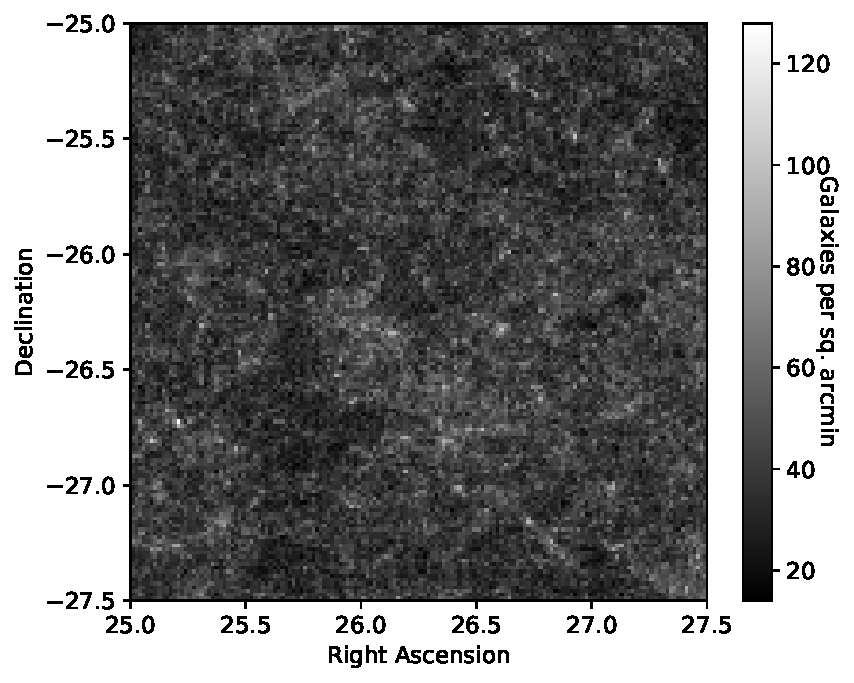
\includegraphics[width=\columnwidth]{figures/galaxies.pdf}
\end{center}
\caption[]{
The distribution of simulated galaxies. The mean galaxy density is 40 arcmin$^{-2}$. 
\label{fig:galaxies}}
\end{figure}

\begin{figure}
\begin{center}
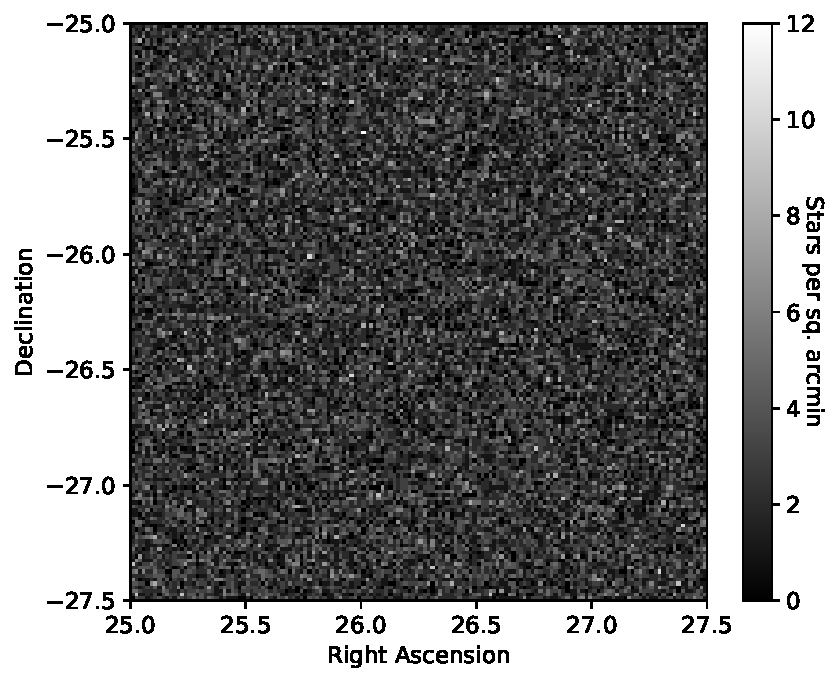
\includegraphics[width=\columnwidth]{figures/stars.pdf}
\end{center}
\caption[]{
The distribution of simulated stars. The mean stellar density is 2.5 arcmin$^{-2}$. 
\label{fig:stars}}
\end{figure}

\begin{figure*}
\begin{center}
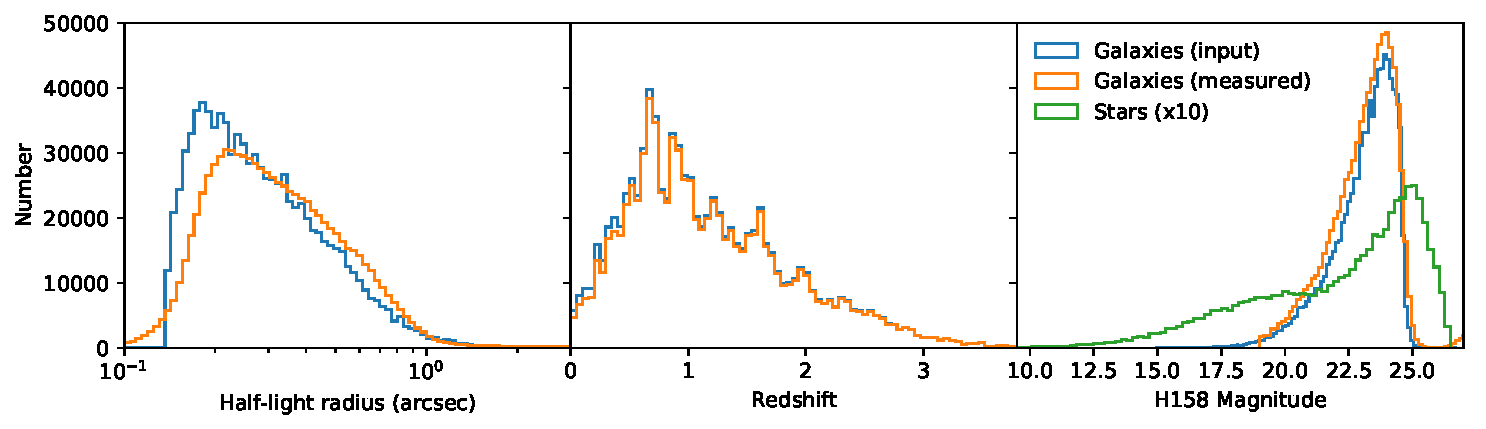
\includegraphics[width=\textwidth]{figures/hist.pdf}
\end{center}
\caption[]{
The input distributions of half-light radius, redshift, and H158 magnitude for galaxies (blue) and stars (orange). 
\label{fig:hist}}
\end{figure*}

\begin{figure}
\begin{center}
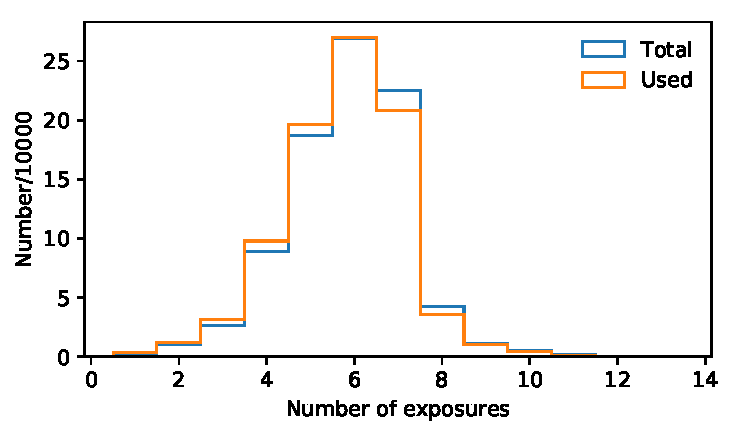
\includegraphics[width=\columnwidth]{figures/hist2.pdf}
\end{center}
\caption[]{
The number of exposures per object simulated (total) compared to the number used in the shape measurement.
\label{fig:hist2}}
\end{figure}

\begin{figure*}
\begin{center}
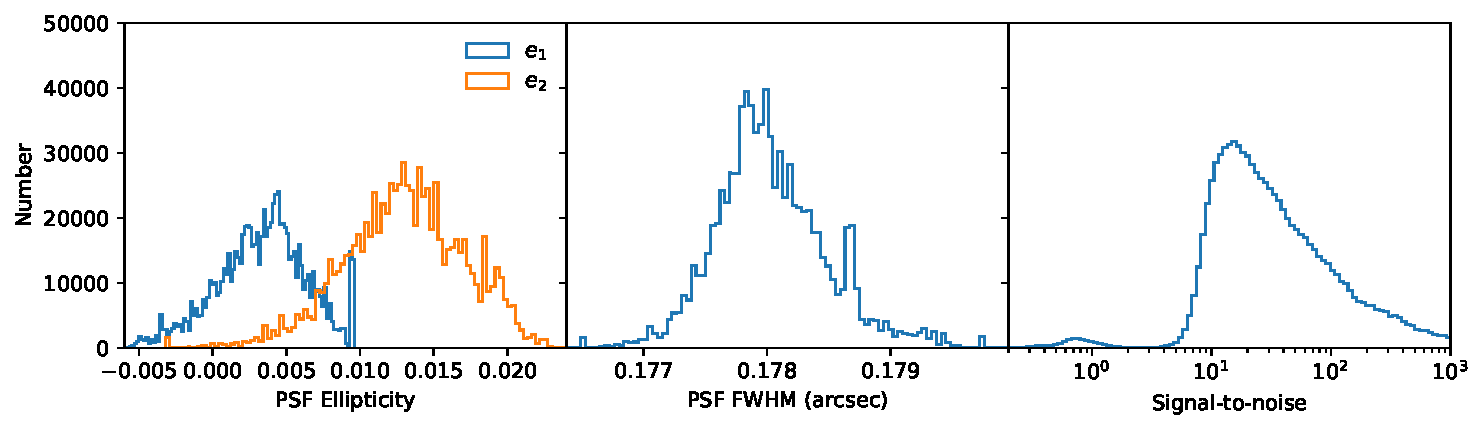
\includegraphics[width=\textwidth]{figures/hist3.pdf}
\end{center}
\caption[]{
The measured PSF ellipticity and size, and the signal-to-noise of the galaxy measurements.
\label{fig:hist3}}
\end{figure*}

\begin{figure}
\begin{center}
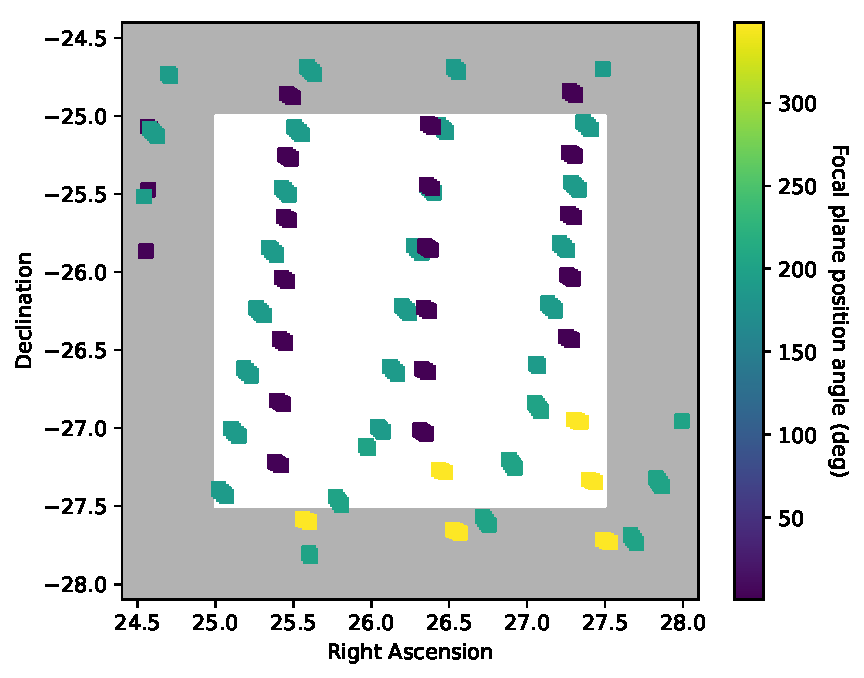
\includegraphics[width=\columnwidth]{figures/pointings.pdf}
\end{center}
\caption[]{
Pointings that overlap the simulated region (non-shaded). The color of each marker shows the position angle of the focal plane.
\label{fig:pointings}}
\end{figure}

\begin{figure*}
\begin{center}
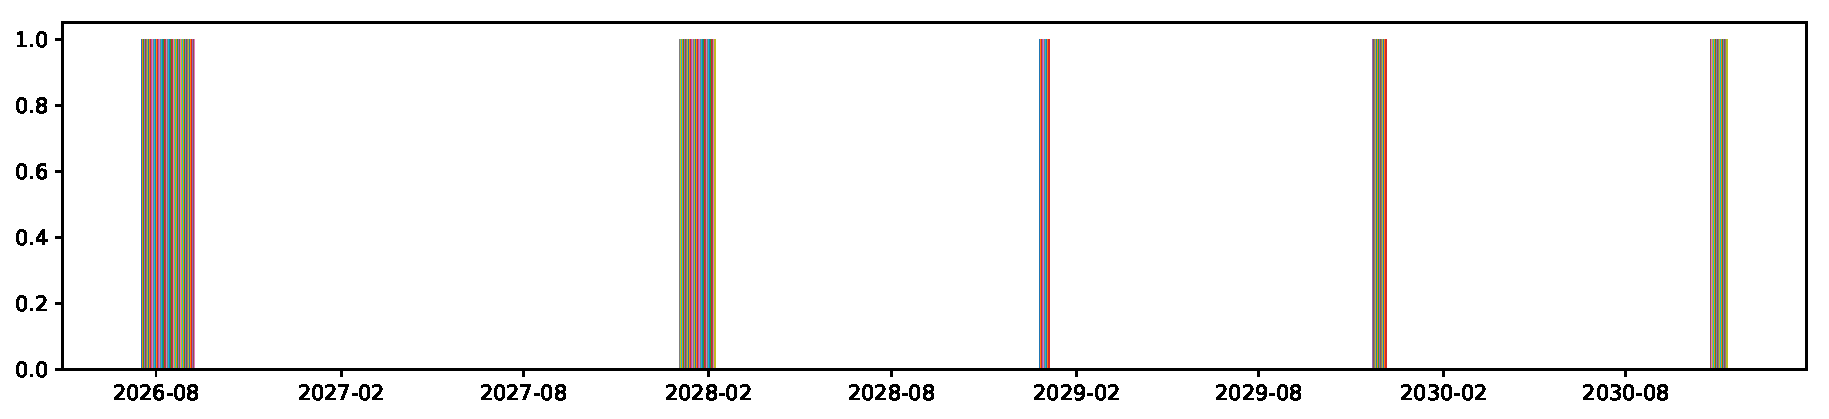
\includegraphics[width=\textwidth]{figures/dates.pdf}
\end{center}
\caption[]{
Dates of observations (is this useful? hard to make it readable)
\label{fig:dates}}
\end{figure*}

\begin{figure}
\begin{center}
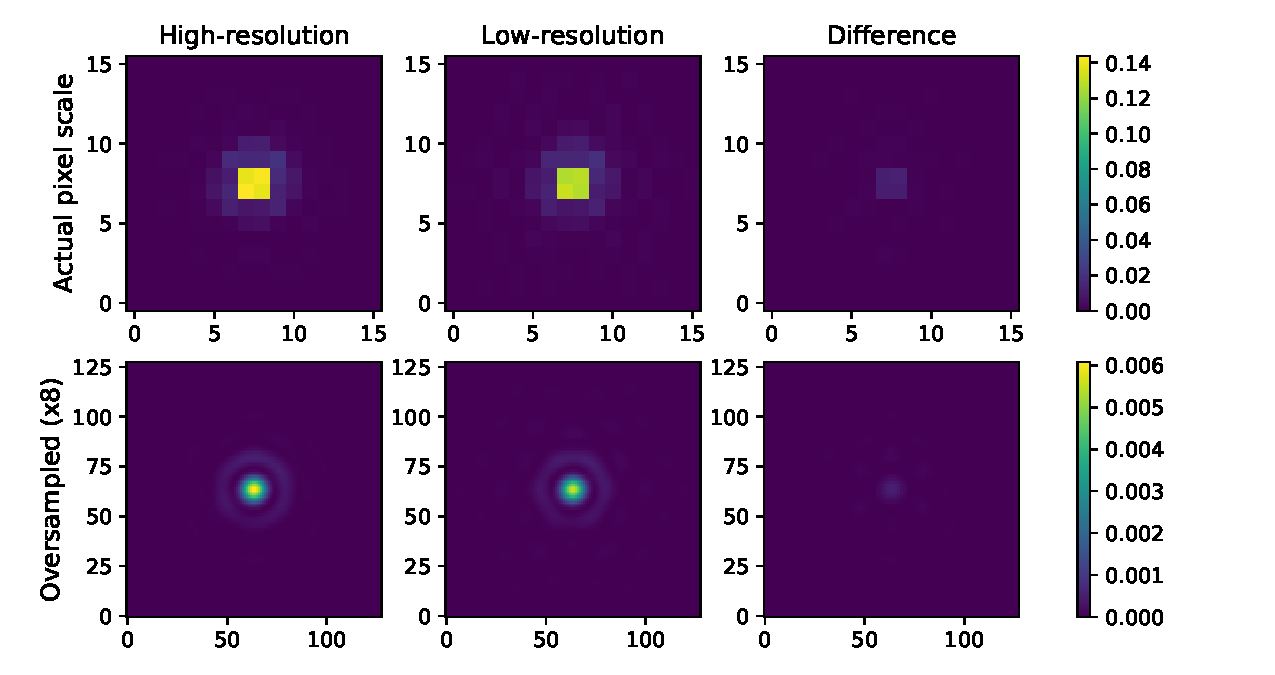
\includegraphics[width=\columnwidth]{figures/psf.pdf}
\end{center}
\caption[]{
PSF model for SCA 1. The top row shows the model in native pixel scale, while the bottom row is oversampled by a factor of 8. From left to right: a comparison of the high-resolution ('true') model, the low-resolution model used in the simulation, and the difference of the two models. The color bars are defined by the range of the high-resolution model.
\label{fig:psf}}
\end{figure}

\begin{figure}
\begin{center}
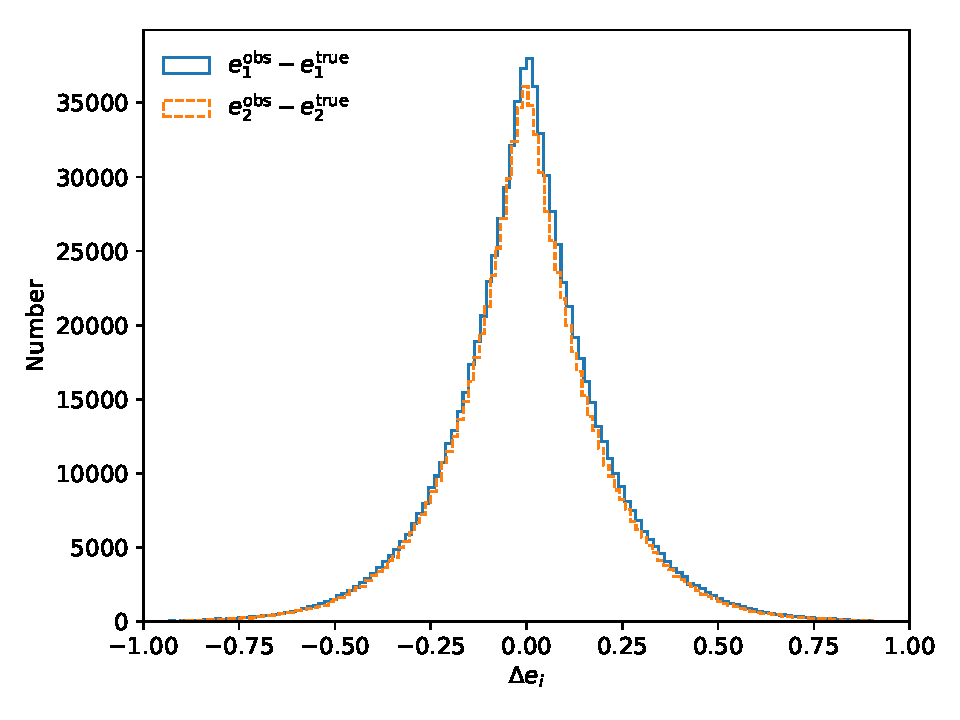
\includegraphics[width=\columnwidth]{figures/shape_hist.pdf}
\end{center}
\caption[]{
A histogram of the difference in the measured shape from the true shape in the Fiducial simulation.
\label{fig:shape_hist}}
\end{figure}

\begin{figure}
\begin{center}
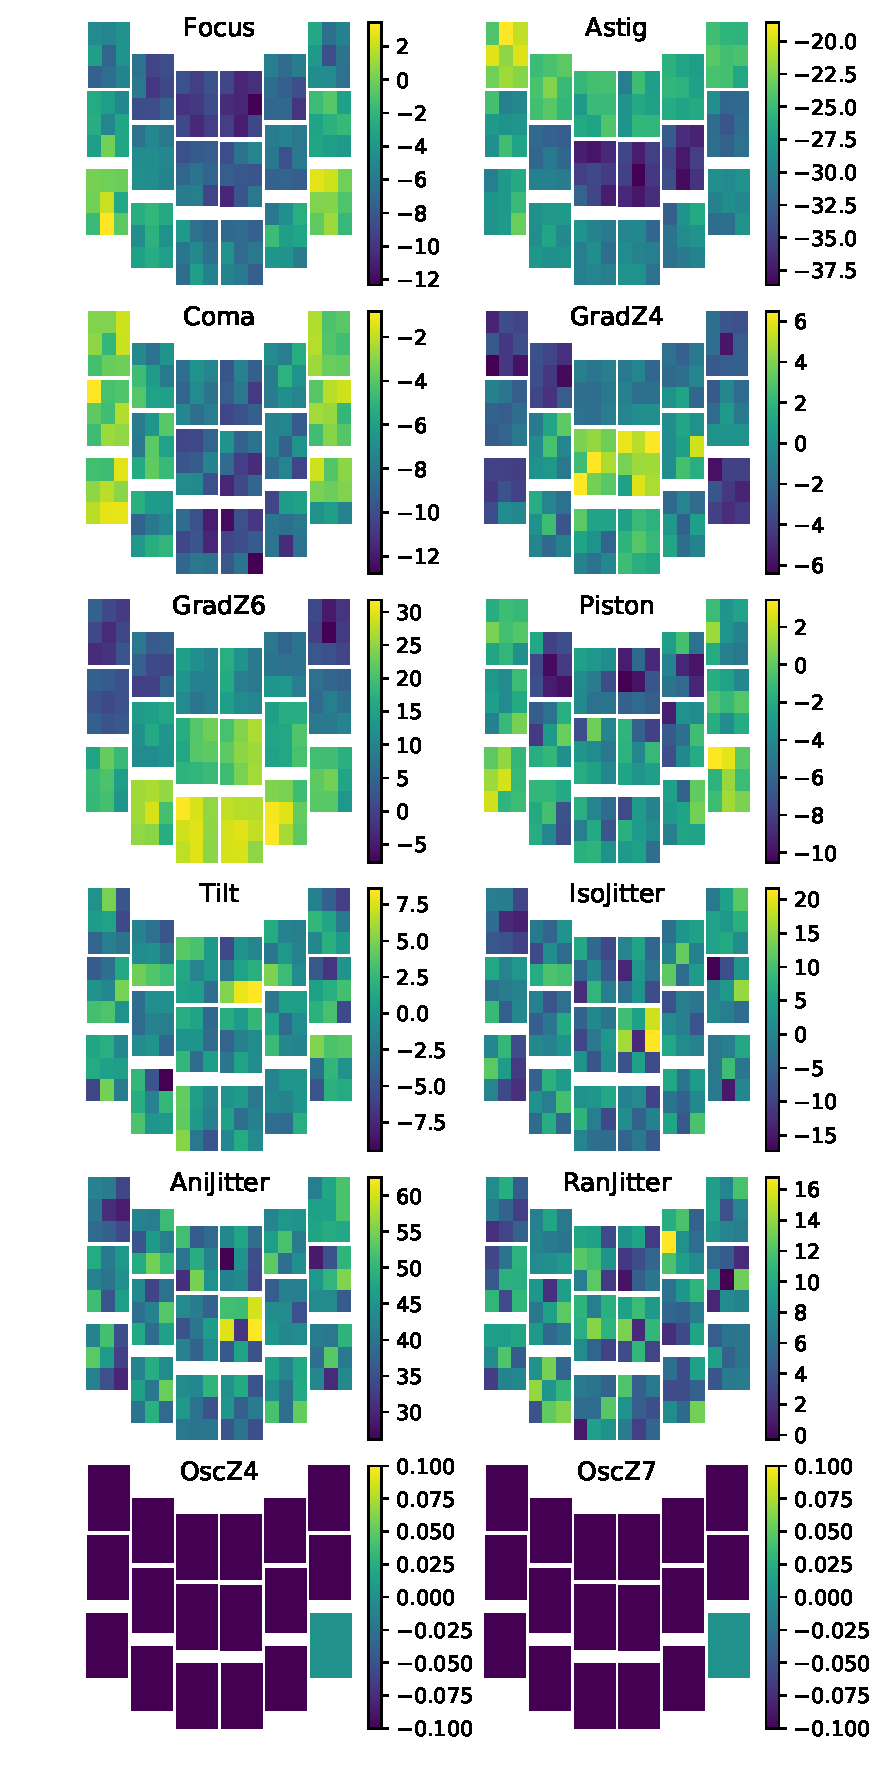
\includegraphics[width=\columnwidth]{figures/focal_mean_e1.pdf}
\end{center}
\caption[]{
The binned mean difference in measured $e_1$ compared to the Fiducial run. Each color bar is in units of $1\times 10^-4$.
\label{fig:focal_mean_e1}}
\end{figure}

\begin{figure}
\begin{center}
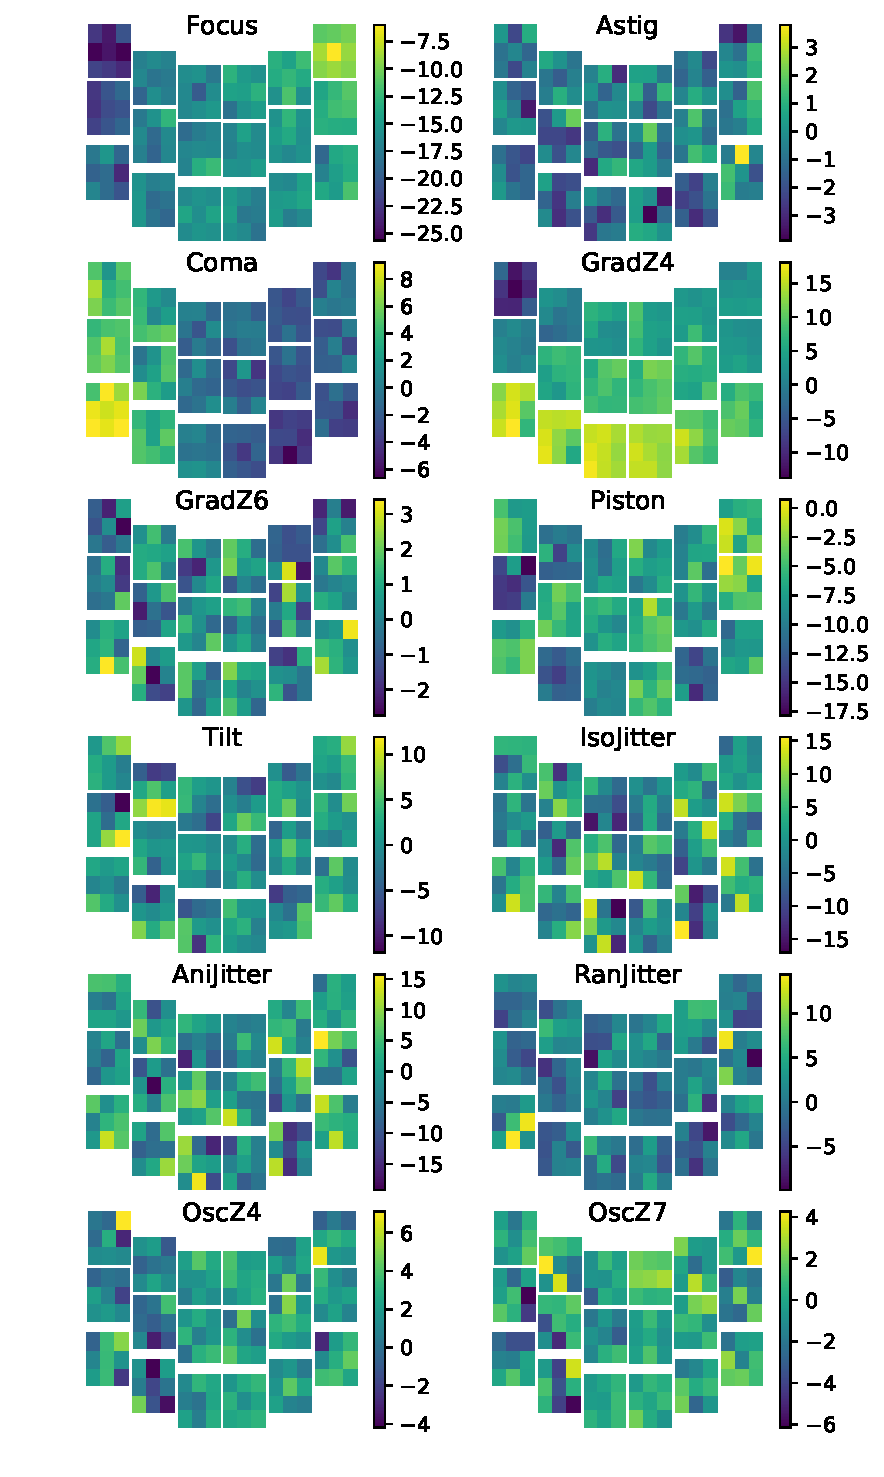
\includegraphics[width=\columnwidth]{figures/focal_mean_e2.pdf}
\end{center}
\caption[]{
The binned mean difference in measured $e_2$ compared to the Fiducial run.  Each color bar is in units of $1\times 10^-4$.
\label{fig:focal_mean_e2}}
\end{figure}


\section{Simulation suite}\label{sec:sim}

\begin{itemize}
\item We have developed a realistic synthetic survey 
\item into to a synthetic survey and necessary components
\item galsim framework and cycle 7 (\verify{6?}) baseline
\item Detailed description of simulation suite components
\end{itemize}

To empirically test weak lensing requirements, methods, and algorithms in WFIRST, we have designed a sufficiently complex synthetic survey that, while not entirely realistic in all object properties, contains sufficiently complex and representative objects as to enable informative tests and preliminary algorithm development. 
This synthetic survey utilizes several external simulation and data sources, and generates WFIRST-like imaging using the \galsim\ framework and its WFIRST module. 
The simulation framework is generally capable of producing a full WFIRST HLS imaging survey in all filters matching Cycle 7 specifications. 
The code is publicly available at \url{https://github.com/matroxel/wfirst_imsim}, where configuration files are provided for the fiducial simulation used in this work.
Figure \ref{fig:fov} shows an example pointing produced in the fiducial simulation, and Fig. \ref{fig:sca} shows a larger view of one of the SCAs. 
Performance details are provided in Appendix \cite{app:performance}. 

\subsection{Simulation stages}\label{stages}

The simulation is broken into several stages:

\textbf{\textit{Truth catalog generation}} -- A truth catalog is generated from the input galaxy distribution, photometric galaxy catalog, and Milky Way simulation. 
The following true object properties are assigned to each galaxy in the input galaxy distribution (from which the unique galaxy id is generated): 
1) The position in RA and Dec from the galaxy distribution; 
2) Photometric properties drawn from a random object in the photometric galaxy catalog (consistent $YJHF$ magnitudes, size, and redshift); 
3) Intrinsic ellipticity components drawn from a Gaussian distribution of width 0.27 (truncated at $\pm$0.7); 
4) A random rotation angle; 
5) The ratio of fluxes in each of the three galaxy components: a) de Vaucouleurs bulge, b) exponential disk, and c) random walk star-forming knots (a maximum of 25\% of flux can exist in the knots); 
6) The gravitational shear applied to the object, drawn from a discrete list of $(e_1, e_2) \in \{\pm 0.1, \pm 0.1\}$, though including a coherent shear field instead is a simple modification. 
Further details on the provenance of the galaxy catalogs and Milky Way simulation can be found in Secs. \ref{galcats} and \ref{starcat}, respectively. 
These truth properties are saved in a light-weight FITS format that is accessed by the following stages.

\textbf{\textit{Image generation}} -- In this stage, an empty SCA image is initialized ($4088\times4088$ pixels), and a model is built for each galaxy and star is turn, then drawn into the image. 
The galaxy models are built chromatically from the truth parameters for the object, with each component being assigned a different representative SED of types: S0 (bulge), SBa (disk), and Im (knots), respectively. 
The assigned SED is the same for all objects, since after redshifting the spectrum and applying the appropriate flux in each component and size, the model is converted to be achromatic in each passband to speed up the drawing.\footnote{This simplification can be removed, however, at the cost of multiple factors of increased runtime.}
The intrinsic ellipticity, random rotation, and gravitational shear is then applied.
For stars, we apply the SED of Alpha Lyra to a chromatic delta function model. 
Stars are also converted to be achromatic before drawing.
Both stars and galaxies are then convolved with the appropriate PSF for the SCA (constant across the SCA in the fiducial simulation). An example of the PSF model for an object is shown in Fig. \ref{fig:psf}. We save images of the true PSF model both at native pixel scale and oversampled by a factor of 8, in stamps of native pixel size $8\times 8$ at the position of each galaxy.

The models are drawn in dynamically-sized squares stamps, the sizes of which are chosen automatically by \galsim\ to include at least 99.5\% of the flux.
These stamps are then added to the SCA image and saved separately (if drawing a galaxy) to provide an isolated image of each simulated galaxy to allow for tests of the impact of blending.
Objects that would have a postage stamp that overlaps the SCA image are drawn, such that light from objects in chip gaps are appropriately drawn onto the SCA, but we only save postage stamps for objects that have a centroid that falls on the SCA. 
We do not save isolated postage stamps of objects that have a stamp size of greater than 288$\times$288 pixels, but they are drawn into the images.
Finally, each isolated postage stamp is processed through the steps described in Sec. \ref{effects} to simulate the WFIRST observatory and detectors and written to disk. When all objects are added to the full SCA image, it is also processed through these steps and written to a FITS image file.
The simulation is parallelized at the SCA level, such that each SCA in each pointing can be run independently. 
(send sentence to appendix) The truth file is lightweight and completion time semi-random, such that even remote disk I/O has not been a limiting factor at the level of thousands of parallel jobs. 

\textbf{\textit{MEDS creation}} -- We then compile the output across pointings of the isolated object stamps into MEDS (Multi-Epoch Data Structure) files\footnote{https://github.com/esheldon/meds}. 
These files concatenate all exposures of unique objects to allow for fast access for object-by-object data processing (like shape measurement). 
Each MEDS file also stores for each object (and stamp) its original SCA, the object position and the stamp position within the SCA, the WCS for each stamp, the PSF model for each object, and other ancillary information. 
Each MEDS file contains all objects within a $n_{\textrm{side}}=512$ Healpixel.

\textbf{\textit{Shape measurement}} -- We utilize the MEDS files to measure the shapes of each galaxy and the PSF. 
The galaxy shape is measured by jointly fitting a two-component model, de Vaucouleurs bulge and exponential disk, across all suitable exposures. 
Exposures where more than 20\% of the pixels are masked (i.e., the centroid falls too close to the edge of the SCA) are rejected. 
The model fit has x parameters: $e_{1,2}$, $p_{x,y}$, half-light radius, flux, and bulge flux fraction, where $e_{1,2}$ is the component of the ellipticity and $p_{x,y}$ is the pixel centroid offset. 
The fits are done using the \textsc{ngmix}\footnote{https://github.com/esheldon/ngmix} and \textsc{MOF}\footnote{https://github.com/esheldon/mof} packages \cite{2014MNRAS.444L..25S}. 
We also measure the PSF size and shape using an adaptive moments method \cite{2003MNRAS.343..459H}. 
This stage writes a set of FITS files containing the galaxy and PSF measurement results and relevant truth catalog information.

\subsection{\galsim}

As mentioned above, the image rendering uses the \galsim\ software package \cite{Rowe15}.  
This package has been extensively tested and has been shown to yield very accurate rendered images of galaxies and stars.
Notably, the image rendering process has been shown to impart biases in the shapes of galaxies at a level much less than $10^{-3}$ for the kinds of objects we are simulating here.  

The \galsim\ package is mostly generic with respect to the telescope and observational strategy, allowing for a wide variety of options in performing the simulation.
However, it does have a sub-module (\texttt{galsim.wfirst}) that has a number of WFIRST-specific implementation details.
Some of the code in this module pre-dates this work, but some of it was developed specifically for this project, especially updating some of the details to match Cycle 7 information, and to reflect new information from laboratory tests of persistence in WFIRST sensors.  
The values used for this project correspond to the \texttt{galsim.wfirst} module in \galsim\ release version 2.2.0.
\mj{Note: We should reference a real version number for all this.  The code used was technically master branch when Troxel ran it, but we should tag it as an official release soon, which will match all the important aspects of what Troxel used.}

\subsubsection{World coordinate system}\label{wcs}

The \texttt{galsim.wfirst} module has code to provide an estimate of the WFIRST WCS (world coordinate system) for each SCA given a rotation angle, date, and pointing direction.  
The WCS gives the two-dimensional mapping from $(x,y)$ coordinates on the image to right ascension (RA) and declination (Dec) on the sky.
The specific orientations and gaps between the sensors was updated to match the Cycle 7 data as part of the development work for this project.
\mj{ref?}

We create our scene of objects in sky coordinates (RA, Dec).
All surface brightness profiles in \galsim\ are defined in sky coordinates as well, so units for things like the half-light radius are typically arcseconds.
We then use a series of pointings and rotation angles designed to match a plausible WFIRST observational schedule. 
\mj{Probably say more about this?  Chri's observing sequence of pointings and such. Or maybe you already did elsewhere.}
\galsim\ is then able to turn these observational parameters into full WCS functions for all 18 SCAs and determine which objects in the scene would be observed by each sensor.

\galsim\ automatically accounts for the Jacobian of the WCS transformation when rendering the surface brightness profiles on each sensor's pixels.  
Details such as the telescope distortion and variable pixel area are correctly accounted for in this process.

\subsubsection{Point-spread function}\label{psf}

For the point-spread function (PSF) we use a model of the WFIRST PSF from the \texttt{galsim.wfirst} module.
While this module includes a high-resolution Cycle 7 estimate of the WFIRST spider pattern (i.e. the obscuration of the struts and camera in the pupil plane), we use a faster, low-resolution approximation, which gets the qualitative features correct, but has a slightly different detailed diffraction pattern.  
For the purposes of this study, we are insensitive to the differences between the two spider patterns, so we did not enable the slower, more accurate option.
%%%MJ: The below text is right if you aren't using approximate_struts.  But I think you are.
%The spider pattern image for band F184 is slightly different from that in the other two bands (J129 and H158).  
%Technically, the effective spider pattern varies continuously with wavelength, but the difference between the %two shorter wavelength bands is small, and we approximate them as having the same pattern.

The PSF uses positition-dependent (Zernike) aberrations, based on an investigation of the field-dependent wavefront errors for Cycle 5.0.6\footnote{\url{https://wfirst.gsfc.nasa.gov/science/sdt_public/wps/references/instrument/README_AFTA_C5_WFC_Zernike_and_Field_Data.pdf}}.
We are not aware of a more recent update to these numbers.  
Aberrations between the tabulated positions are estimated using bilinear interpolation of the tabulated values.

The wavelength-dependent features of the PSF, such as the width of the Airy diffraction pattern, and the wavelength-dependence of the aberrations, are taken at the effective wavelength of the observation bandpass.
This is an approximation, which leads to an enormous speed up in the rendering time.
However, it does omit some interesting and subtle chromatic effects as different parts of a galaxy, with different effective SEDs, would be convolved by slightly different effective PSFs.
There are plans to improve the implementation of this aspect of \galsim, but it cannot currently simulate such effects efficiently enough for our needs.

There are also plans to enable the use of WebbPSF\footnote{\url{https://webbpsf.readthedocs.io/en/stable/}} in \texttt{galsim.wfirst} to leverage the work being done on that project to simulate the WFIRST PSF.
That PSF is qualitatively similar to what we are using from \texttt{galsim.wfirst}, but there are slight differences.
We expect that the WebbPSF model is probably more accurate, so we look forward to being able to use that in future simulations.

\mj{Both of the above planned improvements will be done by us.  (Probably me in fact.)  Not sure if we should allude to that fact or not...}

\subsubsection{Implemented detector effects}\label{effects}

Most of the development of \galsim\ has been to render simulations of CCD images.
The HgCdTe detectors used by WFIRST are qualitatively similar, but there are significant differences in the physics, which lead to differences in some of the simulation steps.

Reciprocity failure is a non-linear relationship between the voltage response in the detector to the incident flux of photons at low light levels.
The exact mechanism of this effect is unknown and hence we lack a good theoretical model. 
\galsim\ uses a power law
\begin{equation}
\frac{p}{p_\mathrm{nominal}} =
 \left(\frac{p_\mathrm{nominal}}{f_0 t_\mathrm{exp}}\right)^{\frac{\alpha}{\log(10)}}
\end{equation}
where $p_\mathrm{nominal}$ is the pixel response (in electrons) that would have occurred in the absence of reciprocity failure,
$p$ is the actual observed response due to reciprocity failure,
$f_0$ is the base flux rate (in electrons/sec) at which the nominal gain was calibrated, 
$t_\mathrm{exp}$ is the exposure time,
and $\alpha$ is taken to be $6.5 \times 10^{-3}$ for the WFIRST sensors.

A particularly pernicious effect present in the HgCdTe detectors is known as ``persistence''.  
In a series of images taken sequentially, some small fraction of the charge accumulated in earlier exposures apparently remains in the sensor and appears in later exposures.  
The effect lasts for many minutes across multiple reset cycles.  
Therefore, for simulating the effect, we need to keep track of the precise order of the observations, the time of each, and the electron-level (i.e. pre-read-out) images of multiple prior exposures.

The exact functional form of this effect is not very well understood, although some progress is being made in laboratory tests.  
The functional form for this effect was updated during the Cycle 7 updates to account for recently improved understanding from laboratory measurements.
\galsim\ now uses a fermi profile when the deposited flux is above the half-well level, and linear below.
Above the half-well, the functional form is
\begin{equation}
n_\mathrm{persist} = \frac{A \left(n/n_0\right)^a  \left(\frac{t}{1000 \mathrm{sec}}\right)^{-r}}
{ \exp(- \frac{n-n0}{dn})+ 1}
\end{equation}
where $A$, $n_0$, $a$, $r$, and $dn$ are constants estimated from laboratory measurements (and stored in the \texttt{galsim.wfirst} module).

In addition to the non-linear pixel response, known as reciprocity failure, there is also a non-linearity in the conversion of accumulated charge to the measured voltage.
This is a different effect, which occurs at a different point in the simulation -- namely, after the application of dark current and persistence. 
\galsim\ treats this as a modification in the effective number of electrons:
\begin{equation}
n_e^\prime = n_e - 6 \times 10^{-7} n_e^2
\end{equation}
where $n_e$ is the actual number of electrons accumulated and $n_e^\prime$ is the effective number to account for the voltage response nonlinearity.

Inter-pixel capacitance (IPC) essentially amounts to a convolution of the image by a $3 \times 3$ kernel in pixel coordinates.
However, the timing of the convolution is during the readout process, which means that some (but not all) of the noise has already occurred.  
Thus it cannot be treated as part of the PSF for the purpose of the simulation.  
It needs to be applied separately after the dark current and Poisson shot noise have been applied, but before the read noise.  
The IPC coefficients have been measured in the lab for WFIRST detectors; the values used in the \texttt{galsim.wfirst} module come from the Cycle 5 estimates.

\mj{It looks like there were Cycle 7 updates to these coefficients.  But we don't seem to be using them.  Slightly awkward....}


\subsection{Galaxy catalogs}\label{galcats}

The input galaxy catalog is created using a simulated galaxy distribution on the sky taken from one realization of the Buzzard simulation \cite{2019arXiv190102401D,wechsler2019}, to introduce realistic galaxy clustering. 
Each galaxy is then assigned a random set of photometric properties matching a galaxy from a sample based on the Candels survey that simulates the fiducial WFIRST weak lensing sample selection \cite{2019ApJ...877..117H}. 
We show the galaxy distribution in Fig. \ref{fig:galaxies}. 
We use a galaxy density that is approx. 40 arcmin$^{-2}$. 
In Fig. \ref{fig:hist}, we show the distributions of size, redshift, and H158 magnitude in the Candels sample. 
We discard less than 1\% of the largest objects in the shape measurement stage, however, due to a maximum postage stamp size restriction. 
In general, the input distribution and properties of galaxies can be easily modified by configuration (i.e., specifying a different input galaxy catalog).

\verify{Need lensing selection cuts and maybe short description of candels sample.}

\subsection{Star catalog}\label{starcat}

We simulate the positions and magnitudes in WFIRST bandpasses of input stars using the galaxy simulation Galaxia\footnote{http://galaxia.sourceforge.net} \cite{galaxia}. 
Galaxia uses an analytic model \cite{galaxia2}  to simulate stars in the galaxy that includes a thin and thick disk with warp and flaring, bulge, and halo components. 
Stars are simulated to 27th magnitude in V band, extinction is added, and they are uniformly translated to WFIRST bandpasses using the stellar SED of Alpha Lyra derived from HST CALSPEC and packaged with \galsim. 

\subsection{Survey strategy}
\assign{Hirata}

\subsection{Simulation implementation for this study}

In this work, we are interested in the impact of how a variety of biases in the PSF model propagate to shape measurement and the weak lensing signal. 
To study this, we produce a set of 13 image simulations that are identical, including noise, modulo a single PSF model change relative to the fiducial simulation in each case. 
The details of these changes and their impacts are described in more detail in Sec. \ref{results}. 
Shape measurement is then performed on the images with some PSF model bias, but using the fiducial, unbiased PSF model for deconvolution, to simulate an unknown wavefront error.

Several simplifications are employed relative to the generic synthetic survey generation described in Sec. \ref{stages} to accommodate the computational load of the many realizations of the survey we are producing. 
\begin{itemize}
\item We simulate objects in a 2.5$\times$2.5 deg$^2$ patch of the sky.
\item We only simulate pointings targeted for the H158 filter. 
Since we are not simulating chromatic effects, the specific filter choice does not make a large difference in our results. 
\verify{This will have an impact on the 'averaging' of PSF errors, however, ...need justification or explanation} 
\item We use a lower-resolution version of the PSF, which significantly speeds up the convolution.
The impact of this approximation on the PSF model, in both native and oversampled pixels, can be seen in Fig. \ref{fig:psf}. 
\item To better isolate the effects of PSF changes, we only utilize the isolated object postage stamps in shape measurement.
\item We do not simulate objects with photometry that would fall below the fiducial weak lensing selection criteria.
\item We do not implement a shear calibration scheme like metacalibration, since we only care about changes to the recovered shape between simulation runs.
\end{itemize}

We simulate a total of 907,170 unique galaxies and 56,128 unique stars across 189 pointings in each of the runs. The distribution of PSF properties and exposures per galaxy are shown in Fig. \ref{}.

\def\arraystretch{1.4}
\setlength{\tabcolsep}{4pt}
\begin{table}
\caption{Table} A summary of the 13 simulation runs. (+ means done)
\label{table:values}
\begin{center}
\begin{tabular}{lcccc }
\hline
\hline
Run name & PSF change & Mode & Notes \\ 
\hline
Fiducial              & -- & -- & -- \\
Focus                & $Z_4$ & Static & --  \\
Astig                  & $Z_5$ & Static &  -- \\
Coma                & $Z_7$ & Static &  -- \\
GradZ4             & $Z_4$ & Static & Gradient in focal plane  \\
GradZ6              & $Z_6$ & Static &Gradient in focal plane    \\
Piston 		 & $Z_4$ & Static  &Random per SCA   \\
Tilt 			 & $Z_4$ & Static & Random gradient per SCA \\
IsoJitter 		& Gaussian  & High-Freq. & Isotropic  \\
AniJitter 		 & Gaussian & High-Freq. & Anisotropic  \\
RanJitter 		 & Gaussian & High-Freq. & 15\% of pointings  \\
OscZ4 		 & $Z_4$ & Low-Freq. & Time-dependent  \\
OscZ7 		 & $Z_7$ & Low-Freq. & Time-dependent  \\
\hline
\hline
\end{tabular}
\end{center}
\end{table}


\section{Wavefront model errors}\label{sec:results}

\begin{itemize}
\item background on psf and wavefront errors
\item details of wfirst psf in cycle 7 (\verify{6?}) baseline
\item summary of approach 
\end{itemize}

In this paper, we focus on empirical tests of weak lensing requirements for wave front model control (i.e., the PSF) in WFIRST. \verify{Chris: insert text connecting to early motivation section when written}. 

We simulate 13 identical 2.5$\times$2.5 deg$^2$ HLS survey cutouts: a fiducial survey that represents perfect knowledge of the PSF and 12 iterations to simulate failure modes in the PSF reconstruction. 
These are split into three types of failure modes: 1) static biases in the model, which are constant as a function of time, 2) high-frequency biases in the model, which correspond to rapidly changing conditions compared to the timescale of a single exposure, and 3) low-frequency biases in the model, which change over lifetime of the mission, but can be considered static over the timescale of a single exposure. 
In each mode, the (rms) amplitude of the bias corresponds to 0.005 wavelengths (a fiducial wavelength is taken to be 1293 nm), which is equivalent to approx. 6.5 nm. 
\verify{Chris: connect value back to requirement discussion when written.} These runs are summarized in Table \ref{table:runs}.

\subsection{Static biases}\label{sec:static}

We simulate seven static sources of bias in the PSF model. 
Three of these simulations include a coherent change in the PSF model Zernike coefficients, where the fiducial value is changed by 0.005 wavelengths in each of defocus ($Z_4$) -- \emph{Focus}, oblique astigmatism ($Z_5$) -- \emph{Astig}, and vertical coma ($Z_7$) -- \emph{Coma}. 
Two simulations include a coherent gradient in the defocus ($Z_4$) -- \emph{GradZ4} -- and vertical astigmatism ($Z_6$) -- \emph{GradZ6} -- across the focal plane with equivalent rms of 0.005 wavelengths. 
For speed, these are simulated such that the PSF is constant within a single SCA. Finally, two simulations approximate errors in the mounting of the SCAs: 1) a random vertical mounting offset of up to 0.005 wavelengths is assigned to each SCA  -- \emph{Piston}, and 2) a random tilt in the x or y direction is assigned to each SCA  -- \emph{Tilt}, with equivalent rms of up to 0.005 wavelengths. 
These are modeled as changes in the $Z_4$ coefficient, with the PSF being evaluating based on the object $x$--$y$ position within the SCA (i.e., each object assigned a different PSF consistent with this random tilt of the SCA). 
Potential correlated biases in the WCS model due to these changes are ignored in this work, but should be considered in future studies of the WCS model recovery.

\subsection{High-frequency biases}\label{sec:low}

Three high-frequency resonant modes are simulated to represent residual vibrations of the telescope after orienting to a new pointing. 
These are represented by an additional convolution of the image with a Gaussian PSF of rms 0.005 wavelengths. We simulate three cases: 1) an isotropic (about the pointing axis) vibration  -- \emph{IsoJitter}, 2) an anisotropic vibration modeled with a shear of $e_2=0.3$ of the Gaussian  -- \emph{AniJitter}, and 3) only applying this asymmetric vibration to a random 15\% of pointings  -- \emph{RanJitter}.

\subsection{Low-frequency biases}\label{sec:high}

Two low-frequency biases are simulated to represent the Zernike coefficients changes caused by thermal drift through exposures. Thermal perturbation propagates to the 4th and 7th Zernike terms ,which we simulate respectively as \emph{OscZ4} and \emph{OscZ7}.
Here we generate a random time-dependent function $f(t)$ following a power spectrum to quantify  the perturbation of Zernike terms. The power spectrum of thermal drift noise is in the form of a Lorenzian function $P(\nu)=\frac{A}{1+(\nu/\nu_0)^2}$. Here, $A$ is a normalization factor. As the rms amplitude of bias is 0.005 wavelength, which is approximately $\sigma=$6 nm, so $Var f(t) = \sigma^2 $. Also, $Var f(t)=\int_{-\infty}^{+\infty}P(\nu)d\nu=\pi A\nu_0$. Thus, $A=\frac{\sigma^2}{\pi\nu_0}$, with $\nu_0=\frac{1}{2\pi\tau}=3.14\times10^{-4}Hz$ as the time constant $\tau=1hr$. 
\section{Results}\label{sec:results}

Each simulation is analyzed in an identical way, except that shape measurement for each simulation assumes the Fiducial PSF model is the true model, which introduces varying levels of bias. 
All estimates of the multiplicative and additive bias will be explored relative to the Fiducial simulation run, since we have not employed a calibration scheme. 
This is justified to first order, since we are only interested in the relative impacts of the PSF model biases.
We find that 3\% of objects are not included in the shape measurement stage in the Fiducial simulation, due to being too large/bright or because too large a fraction of all cutouts are masked (fall off the edge of an SCA) -- see Sec. \ref{stages} for more details on these selections. 

Since the simulated objects have already been pre-selected as objects that should pass the fiducial WFIRST weak lensing selection, we are able to successfully recover a shape fit for more than 99\% of the remaining objects -- a total of 871,841 galaxies. 
We do not make an additional selection on objects that would pass the fiducial WFIRST shape selection based on measured properties, since we expect all objects to be within this selection if we were to simulate all remaining pointings in other bandpasses. 
The recovered multiplicative shear bias is only approx. 2\% smaller and the mean shear is unchanged if we make this selection, which removes an additional 35\% of objects, almost exclusively due to the signal-to-noise cut. 

We present results for the non-Fiducial simulations only for objects that lie in the intersection of successful shape measurement between each simulation and the Fiducial simulation, to allow for 1-1 comparison of the shapes and cancellation of shape noise and sources of photon noise, which are identical in each simulation. 
We neglect the impact of selection biases here, since implementing a calibration scheme to correct them for objects with an undersampled PSF is beyond the scope of this investigation. 
We anticipate this additional bias will be small, however, since the intersection criteria excludes on average only 0.3\% of objects.

\subsection{Summary statistics}

The bias in an ensemble shear measurement is typically characterized in the weak limit by 
\begin{equation}
e_i^{\mathrm{obs}} = (1+m_i) e_i^{\mathrm{true}} + b_i.
\end{equation}
We find the following multiplicative and additive biases in the Fiducial simulation: 
\begin{align*}
m_1 &= -0.0756 \pm 0.0019\\ 
m_2 &= -0.0940 \pm 0.0019\\ 
b_1 &= 0.00120 \pm 0.00017\\
b_2 &= -0.00157 \pm 0.00016.
\end{align*}
The difference in measured shape vs true input shape (intrinsic shape and shear) is shown in Fig. \ref{fig:shape_hist}.

For each simulation, we compare the recovered shear to the Fiducial simulation in several ways. First, we compare the change to the recovered values of $m$ and $b$, along with the changes in the mean galaxy and PSF sizes and ellipticities, where we use the true model PSF images for each simulation and not the biased PSF model used in the shape measurement. 

We will also represent the changes in $m$ and $b$ as a response to the wavefront error in units of nm. 

\begin{table}
\label{table:partials}
\caption{Table} Ellipticities changes with respect to Zernike coefficients for different modes. The units of high-frequency modes, i.e. IsoJitter, AniJitter and Ranjitter are ${milliarcsec}^{-2}$. For all other modes the units are ${nm}^{-1}$.
\begin{center}
\resizebox{\columnwidth}{!}{
\begin{tabular}{ lcc }
\hline
\hline
%Run name & Fiducial  & Focus & Astig & Coma & GradZ4 & GradZ6 & Piston & ilt & IsoJitter &AniJitter & RanJitter & OscZ4 & OscZ7 \\ 

Run name & $\partial e_1/\partial\psi$ & $\partial e_2/\partial\psi$ \\
\hline
Fiducial              & -- & --  \\
Focus                & $-8.7\times 10^{-5} \pm 3.2\times 10^{-6}$ & $-2.5\times 10^{-4} \pm 3.1\times 10^{-6}$  \\
Astig                 & $-4.5\times 10^{-4} \pm 3.1\times 10^{-6}$ & $-1.0\times 10^{-4} \pm 3.0\times 10^{-6}$  \\
Coma                & $-1.0\times 10^{-4} \pm 3.2\times 10^{-6}$ & $3.0\times 10^{-6} \pm 3.1\times 10^{-6}$  \\
GradZ4             & $-8.9\times 10^{-6} \pm 3.0\times 10^{-6}$ & $1.0\times 10^{-4} \pm 2.9\times 10^{-6}$  \\
GradZ6             & $2.2\times 10^{-4} \pm 2.9\times 10^{-6}$ & $4.4\times 10^{-6} \pm 2.8\times 10^{-6}$  \\
Piston 		 & $-5.6\times 10^{-5} \pm 4.8\times 10^{-6}$ & $-1.2\times 10^{-4} \pm 4.8\times 10^{-6}$  \\
Tilt 			& $-3.6\times 10^{-6} \pm 6.3\times 10^{-6}$ & $1.0\times 10^{-5} \pm 6.3\times 10^{-6}$  \\
IsoJitter 		& $1.2\times 10^{-3} \pm 7.2\times 10^{-3}$ & $1.8\times 10^{-3} \pm 7.0\times 10^{-3}$  \\
AniJitter 		& $0.29 \pm 6.9\times 10^{-3}$ & $-1.9\times 10^{-3} \pm 6.8\times 10^{-3}$  \\
RanJitter 	        & $0.049 \pm 3.2\times 10^{-3}$ & $1.7\times 10^{-3} \pm 3.1\times 10^{-3}$  \\
OscZ4 		 & $1.3\times 10^{-5}\pm 3.9\times 10^{-6}$ & $3.0\times 10^{-5}\pm 3.9\times 10^{-6}$  \\
OscZ7 		& $-1.9\times 10^{-6}\pm 4.5\times 10^{-6}$ & $-4.4\times 10^{-6}\pm 4.4\times 10^{-6}$   \\
\hline
\hline
\end{tabular}}
\end{center}
\end{table}

%\begin{table}
%\label{table:values}
%\begin{center}
%\resizebox{\columnwidth}{!}{
%\begin{tabular}{ |c|c|c|c|c| }
%\hline
%\hline
%%Run name & Fiducial  & Focus & Astig & Coma & GradZ4 & GradZ6 & Piston & Tilt & IsoJitter &AniJitter & RanJitter & OscZ4 & OscZ7 \\ 
%Run name & $m_1$ & $b_1$ & $m_2$ & $b_2$   \\
%\hline
%Fiducial              & $ -0.0756 \pm 0.0019$ & $0.00120 \pm 0.00017$ &  $-0.0940 \pm 0.0019$ & $-0.00157 \pm 0.00016$  \\
%Focus                & $-0.0710 \pm 0.0019 $ & $ 0.00064\pm 0.00017$ & $ -0.0896\pm 0.0019 $ & $-0.00315\pm0.00016$   \\
%Astig                & $-0.076 \pm 0.0019 $ & $-0.00171\pm 0.00017$ & $ -0.0931\pm 0.0019 $ & $-0.00162\pm0.00016$    \\
%Coma                & $-0.0769 \pm 0.0019 $ & $0.00054\pm 0.00017$ & $ -0.0954\pm 0.0019 $ & $-0.00155\pm0.00016$   \\
%GradZ4             & $-0.0783 \pm 0.0019 $ & $0.00115\pm 0.00017$ & $ -0.0966\pm 0.0019 $ & $-0.00090\pm0.00016$   \\
%GradZ6             & $-0.0754 \pm 0.0019 $ & $0.00268\pm 0.00017$ & $ -0.0943\pm 0.0019 $ & $-0.00153\pm0.00016$ \\
%Piston 		 & $-0.0896 \pm 0.0019 $ & $0.00083\pm 0.00016$ & $ -0.1089\pm 0.0019 $ & $-0.00232\pm0.00016$   \\
%Tilt 			& $-0.1133 \pm 0.0019 $ & $0.00116\pm 0.00016$ & $ -0.1303\pm 0.0019 $ & $-0.00149\pm0.00016$   \\
%IsoJitter 		& $-0.1164 \pm 0.0019 $ & $0.00123\pm 0.00016$ & $ -0.1333\pm 0.0018 $ & $-0.00153\pm0.00016$ \\
%AniJitter 		& $-0.0870 \pm 0.0019 $ & $0.00553\pm 0.00016$ & $ -0.1054\pm 0.0019 $ & $-0.00158\pm0.00016$ \\
%RanJitter 	& $-0.0884 \pm 0.0019 $ & $0.00195\pm 0.00016$ & $ -0.1066\pm 0.0019 $ & $-0.00154\pm0.00016$   \\
%OscZ4 		 & $-0.08278\pm0.0019$ & $0.0013\pm 0.00016$ & $-0.10050\pm 0.0018$ & $-0.00135\pm 0.00016$  \\
%OscZ7 		& $-0.08761\pm 0.0019$ & $0.00119\pm 0.00016$ & $-0.10529\pm 0.0019$ & $-0.00158\pm 0.00016$  \\
%\hline
%\hline
%\end{tabular}}
%\end{center}
%\end{table}

\begin{table}
\label{table:bias}
\caption{Table} Additive and multiplicative bias parameter changes.
\begin{center}
\resizebox{\columnwidth}{!}{
\begin{tabular}{ lcccc }
\hline
\hline
%Run name & Fiducial  & Focus & Astig & Coma & GradZ4 & GradZ6 & Piston & Tilt & IsoJitter &AniJitter & RanJitter & OscZ4 & OscZ7 \\ 
Run name & $\triangle m_1\times 10^{3}$ & $\triangle b_1\times 10^{4}$ & $\triangle m_2\times 10^{3}$ & $\triangle b_2\times 10^{4}$   \\
\hline
Fiducial              & -- & -- &  -- & --  \\
Focus                & $4.649 \pm 0.237 $ & $ -5.57\pm 0.238$ & $ 4.358\pm 0.228 $ & $-15.87 \pm 0.304$   \\
Astig                & $-0.226 \pm 0.241 $ & $ -29.14 \pm 0.301$ & $ 0.901\pm 0.209 $ & $-0.549 \pm 0.189$    \\
Coma                & $-1.328 \pm 0.259 $ & $ -6.66 \pm 0.262$ & $ -1.469 \pm 0.211 $ & $ 0.224 \pm 0.341$   \\
GradZ4             & $-2.632 \pm 0.267 $ & $ -0.507\pm 0.210$ & $ -2.515\pm 0.228 $ & $ 6.71 \pm 0.423$  \\
GradZ6             & $0.216 \pm 0.226 $ & $ 14.72 \pm 0.624$ & $ -0.216\pm 0.226 $ & $ 0.441\pm 0.227$ \\
Piston 		 & $-13.596 \pm 4.986 $ & $ -3.70 \pm 0.313$ & $ -14.972\pm 5.256 $ & $-7.51 \pm 0.34$   \\
Tilt 			& $-37.978 \pm 8.044 $ & $ -0.403 \pm 0.382$ & $ -36.629\pm 7.996 $ & $ 0.731 \pm 0.381$   \\
IsoJitter 		& $-40.797 \pm 8.612 $ & $ 0.244\pm 0.835$ & $ -39.489\pm 8.549 $ & $0.425 \pm 0.905$ \\
AniJitter 		& $-11.399 \pm 1.057 $ & $43.27 \pm 0.845$ & $ -11.473\pm 0.958 $ & $ -0.132 \pm 0.857$ \\
RanJitter 	& $-12.820 \pm 4.413 $ & $ 7.50 \pm 0.637$ & $ -12.603\pm 4.099 $ & $ 0.326 \pm 0.431$   \\
OscZ4 		 & $-7.172\pm3.070 $ & $ 0.891\pm0.307$ & $-6.513\pm 3.126$ & $2.148\pm0.491$  \\
OscZ7 		& $-12.067\pm  6.832$ & $-0.083\pm 0.308$ & $-11.351\pm6.315$ & $-0.173\pm 0.437$  \\
\hline
\hline
\end{tabular}}
\end{center}
\end{table}
%
%\begin{table}
%\label{table:re_dm}
%\begin{center}
%\resizebox{\columnwidth}{!}{
%\begin{tabular}{ |c|c|c|c|c| }
%\hline
%\hline
%%Run name & Fiducial  & Focus & Astig & Coma & GradZ4 & GradZ6 & Piston & Tilt & IsoJitter &AniJitter & RanJitter & OscZ4 & OscZ7 \\ 
%Run name & $\triangle m_1/m_{1fid}\times 10^{3}$ & $\triangle m_2/m_{2fid}\times 10^{3}$ & $\triangle b_1/b_{1fid}$ & $\triangle b_2/b_{2fid}$   \\
%\hline
%Fiducial              & -- & -- &  -- & --  \\
%Focus                & $5.029 \pm 0.257 $ &  $ -4.809\pm 0.254 $ & $ -0.462862\pm 0.055216$ & $ 1.01220 \pm 0.111853$   \\
%Astig                & $-2.44 \pm 0.260 $ &  $0.994\pm 0.231 $ & $ -2.420371 \pm 0.291650 $ & $ 0.034980 \pm 0.012969$    \\
%Coma                & $-1.436 \pm 0.281 $ &  $ -1.622 \pm 0.233 $ & $ -0.552890 \pm 0.068065$ & $ -0.014333 \pm 0.021670$   \\
%GradZ4             & $-2.847 \pm 0.289 $ &  $ -2.775\pm 0.251 $ & $ -0.042084 \pm 0.018697$ & $-0.417965 \pm0.051765$  \\
%GradZ6             & $ 0.233 \pm 0.244 $ &  $ -0.337\pm 0.236 $ & $ 1.222809 \pm 0.160794$ & $ -0.026453 \pm 0.014106$ \\
%Piston 		 & $-15.100 \pm 5.402 $ &  $ -16.524\pm 5.805 $ & $ -0.307647 \pm 0.041169$ & $ 0.479172 \pm 0.056785$   \\
%Tilt 			& $-41.084 \pm 8.696 $ & $ -40.428\pm 8.822 $ & $ -0.033508 \pm 0.031404$ & $ -0.046589 \pm 0.002347$   \\
%IsoJitter 		& $-44.134 \pm 9.314 $ & $ -43.584\pm 9.439 $ & $ 0.020227 \pm 0.069474$ & $-0.027127 \pm 0.056551$ \\
%AniJitter 		& $ -12.332 \pm 1.129 $ & $ -12.663\pm 1.050 $ & $ 3.594399 \pm 0.441964$ & $ 0.00838 \pm 0.054719$ \\
%RanJitter 	& $-13.869 \pm 4.774 $ & $ -13.911\pm 4.525 $ & $ 0.622797 \pm 0.095830$ & $ -0.020775 \pm 0.027366$   \\
%OscZ4 		 & -- & --&--&--  \\
%OscZ7 		&-- & -- &--&--  \\
%\hline
%\hline
%\end{tabular}}
%\end{center}
%\end{table}


\subsection{Spatially-Correlated biases}

We are also interested in the spatial correlation of any biases, since this will propagate into the measured shear correlation functions. ...

\begin{figure}
\begin{center}
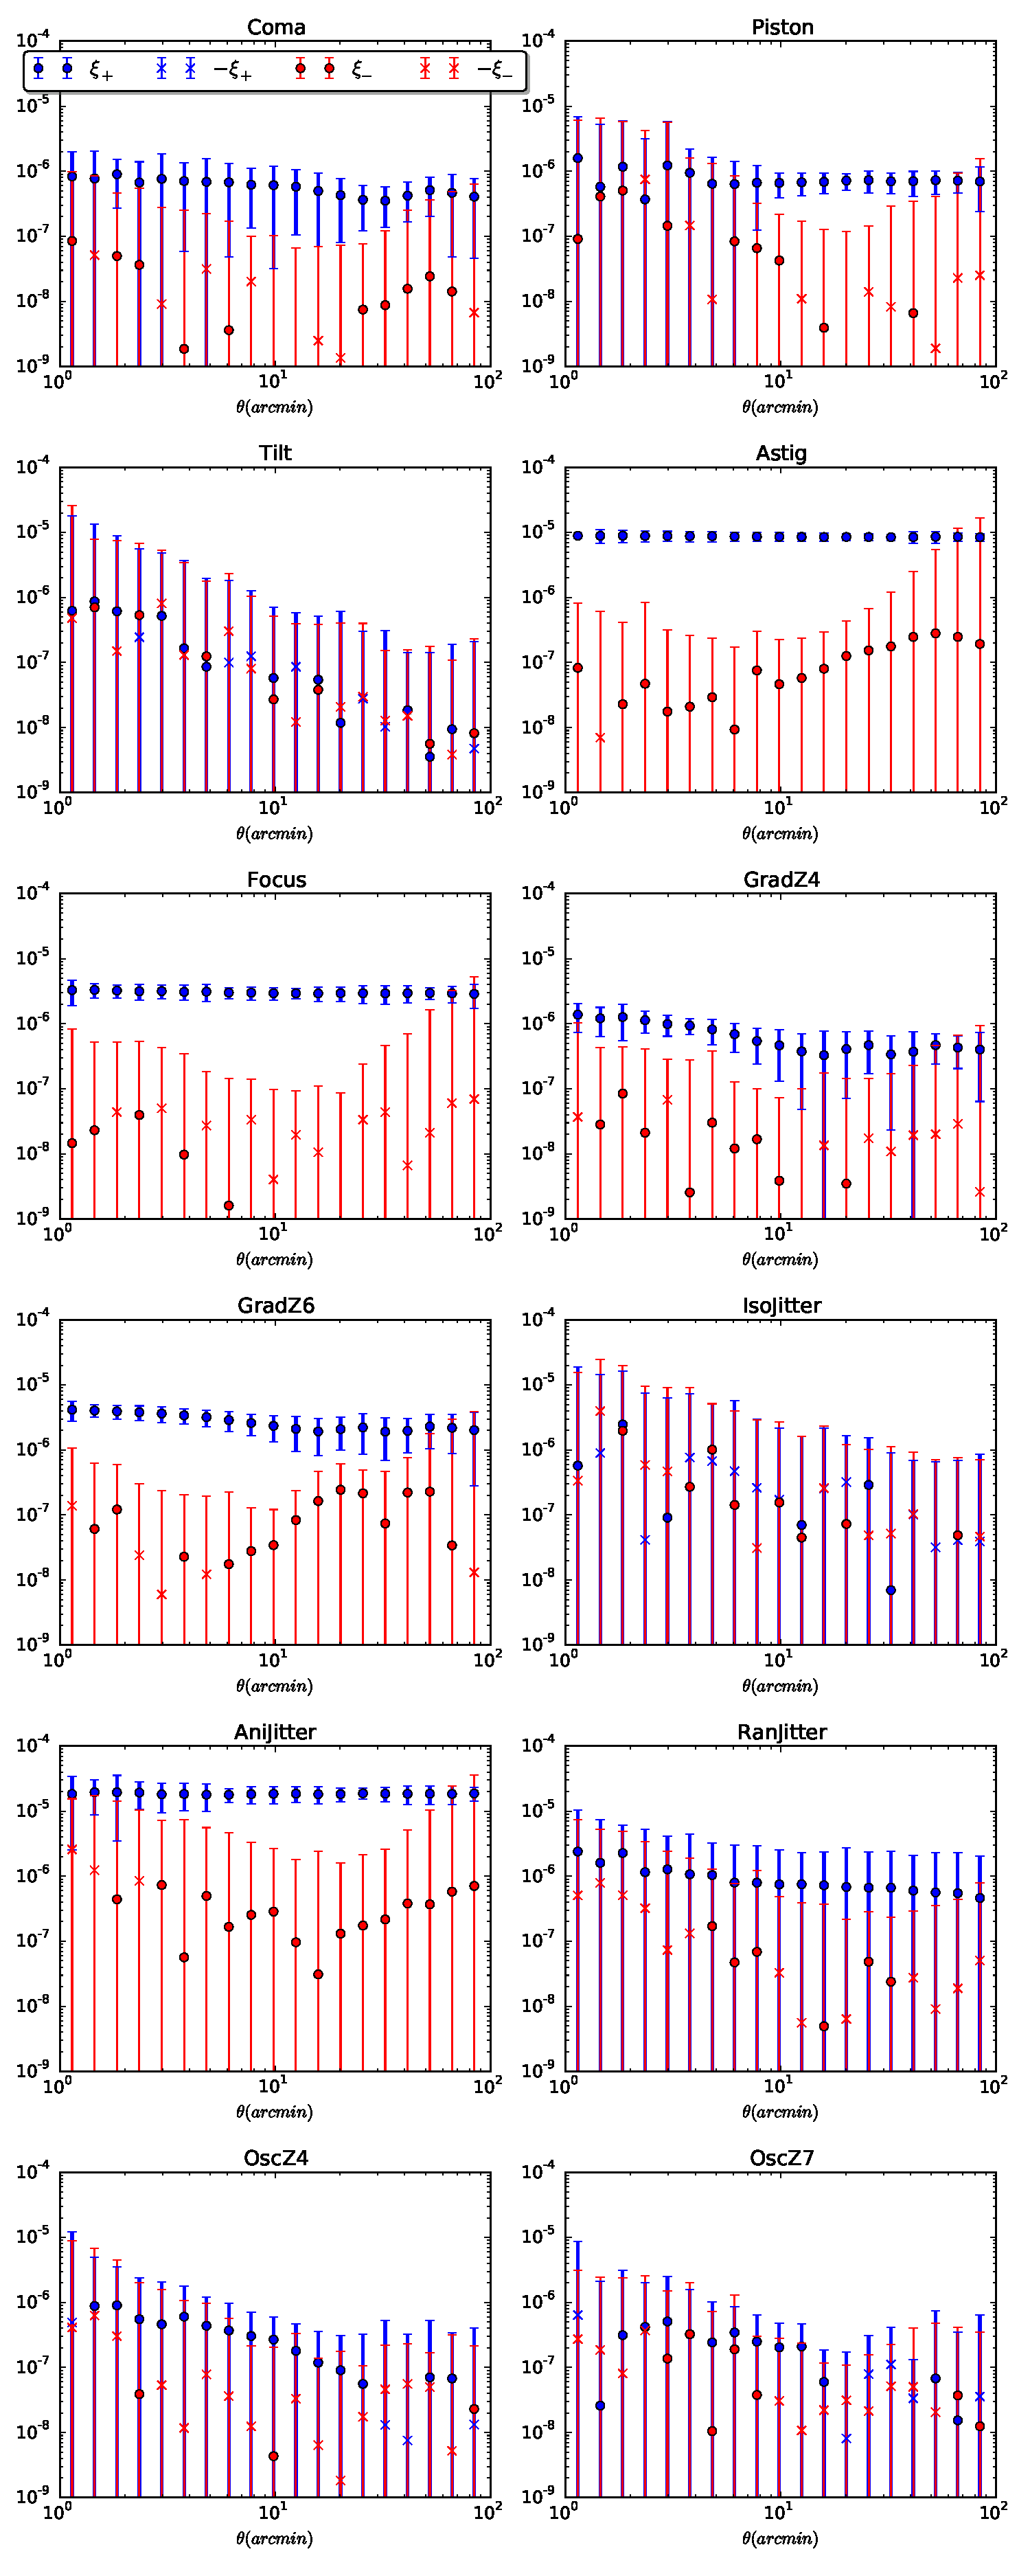
\includegraphics[width=\columnwidth]{figures/2pt_corrs.pdf}
\end{center}
\caption[]{ The correlation function of ellipticity difference between PSF runs and fiducial run. Blue, red points show the two correlation functions measured in sky coordinates: $\xi_{\pm}(\theta)=<\Delta e_1\Delta e_1>\pm<\Delta e_2\Delta e_2>.$
\label{fig:f2pt_corrs}}
\end{figure}

\subsection{Fiducial simulation results}\label{sec:results}

\section{Conclusion}\label{sec:conclusion}

wrap-up

future work and timeline

\section*{Acknowledgements}

This work used resources on the CCAPP condo of the Ruby Cluster at the Ohio Supercomputing Center \cite{OhioSupercomputerCenter1987} and ...OSG, Duke.... Plots in this manuscript were produced partly with \textsc{Matplotlib} \cite{Hunter:2007}, and it has been prepared using NASA's Astrophysics Data System Bibliographic Services.

\appendix

\begin{widetext}

\chris{assorted material on analytic flowdown here. this is material from the appendices the WFI Calibration Plan (the relevant parts were written by me, with some commentary from people I should add to the acknowledgements), with data from the wlrequirements github. this was a Phase A snapshot. We can talk about whether numbers should be updated, but my inclination is *not* to do so and just identify the version, since requirements don't update when we revise, e.g., the galaxy population or instrument model (if they do need updating, we should tell the project). I will also clean up some of the references and broken links in here. many can be made shorter in this document than the calibration plan as they refer to standard WL stuff we can just cite. I plan to do some cleanup of this in the next few days, if you want to wait until that is done to read go ahead.}

\section{Overview of weak lensing systematics budgeting}
\label{app:wl-budget}

This appendix describes the requirements flowdown and error budgeting
for the weak lensing program on the WFIRST mission, and documents the
detailed rationale behind the summary requirements listed in the
WFIRST SRD. This kind of error budgeting has been performed elsewhere
in the literature \cite{2008A&A...484...67P,2013MNRAS.429..661M}, but
this document focuses on the error terms relevant to WFIRST. For
example, the PSFs are based on an obstructed pupil with low-order
aberrations rather than using generic formulae involving second
moments (some such formulae, including those used in the JDEM and
WFIRST-IDRM studies, were for Gaussians).

We set most systematics requirements for this mission on the basis of
having systematic errors sub-dominant to statistical errors in the WL
shear power spectra or cross-power spectra (or any linear combinations
thereof). Exceptions to this policy are considered in cases
where meeting the original systematic budget becomes a cost or
complexity driver, or is not possible. Most measurement biases -- including those considered in this paper -- fall
into the ``additive'' or ``multiplicative'' forms (see
\S\ref{ss:add_mult}) and will be treated according to the formalism
therein.

\subsection{Additive and multiplicative biases}
\label{ss:add_mult}

The cosmic shear measurement is sensitive to two major types of
measurement errors. {\em Additive bias} or ``spurious shear'' is a
shear signal that is detected even when none is present. {\em
Multiplicative bias} or ``calibration bias'' is an incorrect response
to a real shear, e.g.\ a shear $\gamma$ is present in the sky but the
measurement yields 1.01$\gamma$. Normally, we think of additive biases
as resulting from mis-estimation of the PSF ellipticity (or its
variation across the sky), whereas multiplicative biases result from
mis-estimation of the size of the PSF. However, detector
nonlinearities, approximations used in the data processing/analysis
pipelines, and uncertainties about the distribution of galaxy
morphologies in the sky can also contribute to both types of
biases. These biases produce an effect on the observed shear:
\begin{equation}
\gamma({\boldsymbol\theta},z;{\rm obs}) = [1+m(z)] \gamma({\boldsymbol\theta},z;{\rm true}) + c({\boldsymbol\theta},z),
\label{eq:gmod}
\end{equation}
where $m$ is the multiplicative bias parameter (possibly
redshift-dependent) and $c$ is the additive bias field. The $E$-mode
shear cross-power spectrum between two redshift bins $z_i$ and $z_j$
is modified in the presence of these biases:
\begin{equation}
C_\ell^{z_i,z_j}({\rm obs}) = (1+m_i)(1+m_j)C_\ell^{z_i,z_j}({\rm true}) + C_\ell^{c_i,c_j},
\label{eq:mod}
\end{equation}
where we write $m_i\equiv m(z_i)$ as a shorthand. To linear order in
the biases, the correction to the power spectrum can be written as
\begin{equation}
\Delta C_\ell^{z_i,z_j} = C_\ell^{z_i,z_j}({\rm obs}) - C_\ell^{z_i,z_j}({\rm true}) = (m_i+m_j)C_\ell^{z_i,z_j}+C_\ell^{c_i,c_j}.
\label{eq:Delta C}
\end{equation}

\subsection{Setting requirements}

We arrange the power spectra are arranged into a vector ${\bf C}$ with
a covariance matrix ${\bf\Sigma}$. For the WL power spectrum, with
$N_z$ redshift bins and $N_\ell$ angular scale bins, there are $N_\ell
N_z(N_z+1)/2$ power spectra $C_\ell^{z_i,z_j}$; hence ${\bf C}$ is a
vector of length $N_\ell N_z(N_z+1)/2$, and ${\bf\Sigma}$ is a matrix
of size $N_\ell N_z(N_z+1)/2 \times N_\ell N_z(N_z+1)/2$. A
contaminant that changes the power spectrum by $\Delta {\bf C}$ can
have its significance assessed by
\begin{equation}
Z = \sqrt{\Delta{\bf C}\cdot{\bf\Sigma}^{-1}\Delta{\bf C}},
\label{eq:alpha}
\end{equation}
which is the number of sigmas at which one could distinguish the
correct power spectrum from the contaminated power spectrum. Note that
as the survey area $\Omega$ is increased, $Z$ will increase as
$\propto\Omega^{1/2}$, and hence contaminants $\Delta{\bf C}$ must be
reduced to keep them below statistical errors. If $Z=1$, then the
power spectrum is biased at the same level as the statistical
errors. We use $Z$ as a metric for contaminants, rather than
e.g. biases in $(w_0,w_a)$-space, for generality: if $Z<1$ then the
bias due to $\Delta{\bf C}$ in {\em any} cosmological parameter from
the combination of the WFIRST WL power spectrum with {\em any} other
data set(s) from WFIRST or other experiments is $<1\sigma$; whereas if
one based the analysis on biases in $(w_0,w_a)$ then we would need a
separate requirement derived from every cosmological analysis planned
on WFIRST WL data. Using $Z$ as a metric also enables us to write
requirements that do not depend on other cosmological probes (e.g.\
the WFIRST WL systematic error budget does not change if we discover a
new way to reduce the scatter in the SN Ia Hubble diagram), which will
help to ensure the stability of our requirements going forward.

Technically the above discussion applies only to the $E$-mode of
spurious shear; we have not set a specific requirement on the
$B$-mode, which contains no cosmological information to linear order
and is used as a null test. For the latter reason, we set a
requirement on the $B$-mode that is equal to the requirement on the
$E$-mode, so that the $B$-mode null test will pass if requirements are
met. We also note that the WL analysis includes a range of angular
scales, $\ell_{\rm min,tot}\le \ell \le \ell_{\rm max,tot}$;
requirements apply to sources of systematic error that affect these
scales, i.e.\ are ``in-band'' for the WL measurement. The ``in-band''
qualifier is critical: as an example, pixelization errors can cause
shape measurement errors in galaxies that depend on whether the galaxy
lands on a pixel center, corner, vertical edge, or horizontal
edge. For some shape measurement methods, this error may dramatically
exceed the additive systematic error budget, but it is concentrated at
very small angular scales (multiples of $2\pi$ divided by the pixel
scale $P$, or $2\pi/P = 1.2\times 10^7$). Our requirements are set on
the portion of this power that is within (or mixes into) the band
limit, $\ell\le\ell_{\rm max,tot}$ due to e.g.\ edge effects,
selection effects, etc.

Equation~(\ref{eq:alpha}) still does not completely define a
requirement, since we have not described the redshift or scale
dependence of the spurious shear in question. Neither dependence is
expected to be trivial: errors in PSF models have a greater impact on
shape measurements for higher redshift galaxies, since they tend to be
smaller; and the angular power spectrum of PSF model errors should be
non-white in a survey strategy that ``marches'' across the sky, even
if heavily cross-linked (there may also be a characteristic scale at
the size of the field; for example, a repeating error at the $\sim
0.8\times0.4^\circ$ size of the WFIRST field has reciprocal lattice
frequencies at $\ell = 450$ and 900, so a large scale error in the
instrument PSF model that is ``tessellated'' as we tile the sky will
appear at these frequencies or multiples thereof). At first, we
considered assuming a particular scale and redshift dependence for the
errors, but in order to be conservative we would have to assume the
worst combination of angular and redshift dependences. Many of our
large sources of systematic error, such as PSF ellipticity due to
astigmatism, have predictable dependences (e.g.\ the systematic error
induced in galaxy shears is of the same sign in all redshift bins)
that are far from the worst case, and this could lead to
over-conservatism in the requirements. Therefore we need a more
nuanced approach to the requirements, where the allowed amplitude of
each term in the error budget is informed by the structure of the
correlations it produces.

Our approach to this problem is to write a script that accepts a
specific angular and redshift dependence (``template'') for a
systematic error, and returns the amplitude $A_0$ of the systematic
error at which we would have $Z=1$ (i.e.\ a $1\sigma$ bias on the
most-contaminated direction in power spectrum space). For cases where
the template is not known (or where we have not done the analysis),
the script is capable of searching the space of templates and finding
the most conservative choice, i.e.\ the choice that leads to the
smallest value of $A_0$. The combined results enable us to build an
error tree, where the overall top-level systematics requirement (a
limit on $Z$) can be flowed down to upper limits on each source of
systematic error. Finally, some portions of the systematic error
budget sum in quadrature (``root-sum-square'' or RSS addition) and
others linearly; in this document, we carefully account for which is
which.

\subsubsection{Data vector and covariance model}

We build our data vector for the shear power spectra and cross-spectra. We recognize that weak lensing analyses have shifted to ``$3\times 2$-point'' data vectors containing shear-shear, galaxy-shear, and galaxy-galaxy correlations, and by the time WFIRST the list of standard observables may be even longer. However, for setting requirements on shape measurement, shear-shear provides the most demanding use case, and so for simplicity here we only consider shear-shear.

We use for our data vector the $N_\ell N_z(N_z+1)/2$ power spectra and
cross-spectra. Each $\ell$ is treated separately, so there are
$N_\ell=\ell_{\rm max,tot}-\ell_{\rm min,tot}$ angular bins; we use
$\ell_{\rm min,tot}=10$ and $\ell_{\rm max,tot}=3161$, thereby
covering 2.5 orders of magnitude in scale. WFIRST provides little
cosmological constraining power at the larger scales due both to the
finite size of its survey and due to the large cosmic variance of the
lowest multipoles. The smallest scales are generally not used in
cosmic shear analyses because the baryonic effects are severe (e.g.\
\cite{2008PhRvD..77d3507Z, 2013PhRvD..87d3509Z}). We use $N_z=15$
redshift slices, as shown in Table~\ref{tab:dNdz}, which are chosen by the Exposure Time Calculator \cite{2012arXiv1204.5151H} v17, with the Phase B exposure times ($5\times 140.25$ s in $H$-band). In order to ensure
that WFIRST would not become systematics-limited in an extended
mission, we set the top-level requirement on systematics to $Z=1$ for
a survey of area $\Omega =10^4$ deg$^2$ (3.05 sr).

The power spectra were obtained from {\sc Class}
\cite{2011JCAP...07..034B} using the fiducial cosmology from the
{\slshape Planck} 2015 ``TT,TE,EE+lowP+lensing+ext'' results
\citep{2016A&A...594A..13P}. The shape noise contribution was added to
construct ${\bf C}^{\rm tot}$ according to
\begin{equation}
C^{{\rm tot},z_i,z_j}_\ell = C^{z_i,z_j}_\ell + \frac{\gamma_{\rm rms}^2}{\bar n_i}\delta_{ij},
\end{equation}
where $\bar n_i$ is the mean effective number density in galaxies per
steradian in redshift slice $i$, and $\gamma_{\rm rms}$ is the shape
noise expressed as an equivalent RMS shear per component; we take
$\gamma_{\rm rms} = 0.22$.

We approximate ${\boldsymbol\Sigma}$ using the usual Gaussian
covariance matrix formula,
\begin{equation}
\Sigma[C^{z_i,z_j}_\ell, C^{z_k,z_m}_{\ell'}] = \frac{1}{(2\ell+1)f_{\rm sky}} \delta_{\ell\ell'} [ C^{{\rm tot},z_i,z_k}_\ell C^{{\rm tot},z_j,z_m}_\ell + C^{{\rm tot},z_i,z_m}_\ell C^{{\rm tot},z_j,z_k}_\ell],
\label{eq:SGauss}
\end{equation}
where $f_{\rm sky} = \Omega/(4\pi)$.  The non-Gaussian contributions
to the error covariance matrix are turned off, because since the
FoMSWG \cite{2009arXiv0901.0721A} there has been an ongoing program of
using nonlinear transformations on the data to remove them (e.g.\
\cite{2009ApJ...698L..90N, 2011ApJ...729L..11S}) and
we do not want applications of these novel statistics to WFIRST data
to run into systematic error limits. We also do not include astrophysical systematic errors in ${\boldsymbol\Sigma}$; we envision instead that they will be treated with nuisance parameters in the analysis. Another advantage of this is that the covariance matrix ${\boldsymbol\Sigma}$ is block diagonal in $\ell$-space (it is formally $375720\times375720$ without $\ell$-binning), which makes computations possible on a machine with limited memory. Indeed, in the Gaussian case one may write
%The formal length of the data vector ${\bf C}$ is 378240. However, the inversion of Eq.~(\ref{eq:SGauss}) is accelerated by two realizations: first, that each $\ell$ is independent, so that ${\boldsymbol\Sigma}$ is block-diagonal and the contributions of each $\ell$ to $Z^2$ can be linearly summed. Secondly, the particular form of Eq.~(\ref{eq:SGauss}) allows us to write\footnote{This equation is trivially verified by forming, for each $\ell$, linear combinations of the redshift slices that diagonalize ${\bf C}^{\rm tot}_\ell$.}
\begin{equation}
\Delta{\bf C} \cdot {\boldsymbol\Sigma}^{-1} \Delta {\bf C}
= \sum_\ell \frac{(2\ell+1)f_{\rm sky}}2 \sum_{ijkm}
 \Delta C_\ell^{ij} [C^{{\rm tot}-1}_\ell]_{jk}
 \Delta C_\ell^{km} [C^{{\rm tot}-1}_\ell]_{mi},
\label{eq:sprodform}
\end{equation}
where the matrix inverses are $N_z\times N_z$.

\begin{table}
\caption{The effective number density in each redshift bin, in units of galaxies/arcmin$^{2}$, used for setting requirements. These are {\em per bin}, i.e.\ are $dn_{\rm eff}/dz\times\Delta z$. 
\label{tab:dNdz}}
\center{
\begin{tabular}{cc|cc|cc}
\hline\hline
$z$ & $n_{\rm eff}$ & $z$ & $n_{\rm eff}$ & $z$ & $n_{\rm eff}$ \\
\hline
$0.10\pm0.10$ & 3.62 & $1.10\pm0.10$ & 3.75 & $2.10\pm0.10$ & 1.21 \\
$0.30\pm0.10$ & 2.12 & $1.30\pm0.10$ & 3.17 & $2.30\pm0.10$ & 0.95 \\
$0.50\pm0.10$ & 3.05 & $1.50\pm0.10$ & 2.52 & $2.50\pm0.10$ & 0.82 \\
$0.70\pm0.10$ & 5.90 & $1.70\pm0.10$ & 1.45 & $2.70\pm0.10$ & 0.68 \\
$0.90\pm0.10$ & 2.79 & $1.90\pm0.10$ & 1.68 & $2.90\pm0.10$ & 0.19 \\
\hline\hline
\end{tabular}
}
\end{table}

\subsubsection{Implementation: additive systematics}
\label{ss:implement-add}

\begin{table}
\caption{The requirements for additive and multiplicative systematic errors. There are $N_{\rm band}=4$ additive error bands ranging over a total signal band from $\ell_{\rm min,tot}=10$ to $\ell_{\rm max,tot}=3161$. The fraction of the error budget allocated to each band is also indicated, as are the maximum allowed redshift-independent spurious shear ($A_0^{\rm flat}(\alpha)$, RMS per component), and the maximum scaling factors for redshift dependence, $S_{\rm max,\pm}(\alpha)$ and $S_{\rm max,+}(\alpha)$. There is only one row for the multiplicative errors, since the implementation does not contain an $\ell$ dependence; we quote a requirement on the post-calibration shear multiplicative uncertainty $\sigma_{m,\rm req't}^{\rm flat}$.
\label{tab:addbands}}
\center{
\begin{tabular}{r|rrc|c|rr}
\hline\hline
Band $\alpha$ & $\ell_{\rm min}(\alpha)$ & $\ell_{\rm max}(\alpha)$ & Allocation $Z(\alpha)$ & Sys. err. req't. & $S_{\rm max,\pm}(\alpha)$ & $S_{\rm max,+}(\alpha)$ \\ 
 & & & & $A_0^{\rm flat}(\alpha)$ or $\sigma_{m,\rm req't}^{\rm flat}$ & & \\
\hline
\multicolumn7c{Additive errors} \\
0 & 31 & 99 & 0.2596 & $7.000\times 10^{-5}$ &  8.489 &  2.782 \\
1 & 100 & 315 & 0.2539 & $9.900\times 10^{-5}$ &  5.628 &  2.041 \\
2 & 316 & 999 & 0.2575 & $1.400\times 10^{-4}$ &  3.569 &  1.509 \\
3 & 1000 & 3161 & 0.2538 & $1.900\times 10^{-4}$ &  2.119 &  1.149 \\
% Previous table:
%0 & 31 & 99 & 0.2500 & $6.791\times 10^{-5}$ &  8.876 &  2.878 \\
%1 & 100 & 315 & 0.2500 & $9.697\times 10^{-5}$ &  5.862 &  2.100 \\
%2 & 316 & 999 & 0.2500 & $1.360\times 10^{-4}$ &  3.712 &  1.544 \\
%3 & 1000 & 3161 & 0.2500 & $1.855\times 10^{-4}$ &  2.193 &  1.166 \\
\hline \multicolumn7c{Multiplicative errors} \\
mult &  & & 0.4600 & $3.200\times 10^{-4}$ & 2.186 & 1.140 \\ \hline\hline
\end{tabular}
}
\end{table}

Each additive systematic error is taken to have an angular dependence
given by some template $T_\ell$, and a redshift dependence given by a
set of weights $w_i=w(z_i)$. That is, there is a reference additive
shear $c_{\rm ref}$, with the additive shear in redshift bin $i$ given
by $c(z_i) = w_ic_{\rm ref}$. For example, a systematic error
independent of redshift bin would be specified with $w_i=1$ for all
$i$. The reference signal is taken to have a power spectrum
proportional to the template: $C_\ell^{c_{\rm ref}} = A_0^2T_\ell$,
and the template is normalized so that $c_{\rm ref}$ has variance 1
per component (from in-band fluctuations):
\begin{equation}
\sum_{\ell=\ell_{\rm min,tot}}^{\ell_{\rm max,tot}} \frac{2\ell+1}{4\pi} T_\ell = 1.
\label{eq:Tlsum}
\end{equation}
The additive cross-power spectrum is then
\begin{equation}
C_\ell^{c_i,c_j} = A_0^2 w_iw_jT_\ell,
\end{equation}
and the total RMS per component of the spurious shear in bin $i$ is $A_0|w_i|$.

The additive systematic errors can have various scale dependences. We
therefore consider a suite of $N_{\rm band}$ disjoint angular
templates that cover the shape measurement band. Each template
satisfies the normalization rule, Eq.~(\ref{eq:Tlsum}), and has
$\ell(\ell+1)T_\ell/(2\pi)=$constant:
\begin{equation}
T_\ell^{(\alpha)} = \left[ \sum_{\ell'=\ell_{\rm min}(\alpha)}^{\ell_{\rm max}(\alpha)} \frac{2\ell'+1}{\ell'(\ell'+1)} \right]^{-1} \frac{4\pi}{\ell(\ell+1)}
\times\left\{ \begin{array}{cc} 1 & \ell_{\rm min}(\alpha)\le\ell\le\ell_{\rm max}(\alpha) \\ 0 & {\rm otherwise} \end{array} \right.\!,~\alpha=0,1,...N_{\rm band}-1.
\end{equation}
The current bands are displayed in Table~\ref{tab:addbands}. Each band
$\alpha$ is allowed a contribution to the total error
$Z(\alpha)$. Since there are no statistical correlations between
different $\ell$s in the covariance matrix ${\bf\Sigma}$, the
$Z(\alpha)$ can be quadrature-summed (see
Eq.~\ref{eq:alpha}). However, additive systematic error is positive in
the sense that it adds rather than subtracts power; thus the power
spectrum error vectors $\Delta{\bf C}$ from two sources of additive
systematic error contributing to the same angular bin are not
orthogonal and the $Z$'s should be added linearly. Another way to
think of this is that since $Z$ is proportional to the square of the
RMS shear, $Z\propto A_0^2$, quadrature-summation of the additive
shear is equivalent to linear summation of the $Z$-values.

The allocations for each bin $Z(\alpha)$ were initially set to $\sqrt{0.25/N_{\rm band}}$, so that in an RSS sense 25\%\ of the systematic error budget is allocated to additive shear; with 4 bands this implies $Z(\alpha)=0.25$ (i.e., 6.25\% of the error budget in an RSS sense) for each band. There have been some updates of the exposure times, throughputs, and number densities since the SRD requirements were set (December 2016); we have kept the requirements the same, and updated the $Z$-values, so the latter do not exactly equal 0.25.

The construction of $Z$-values for each angular band and each additive
systematic is mathematically sufficient to build the error
budget. However, they can be difficult to conceptualize. Therefore, we
introduce some equivalent notation to describe the WL error
budget. For each angular template, we introduce a limiting amplitude
$A_0^{\rm flat}(\alpha)$, defined to be the amplitude $A_0$ at which
we would saturate the requirement on $Z(\alpha)$ for bin $\alpha$ in
the case of a redshift-independent systematic $w_i=1\,\forall i$. That
is, if the additive systematics did not depend on redshift, we could
tolerate a total additive systematic shear of $A_0^{\rm flat}$ (RMS
per component) in band $\alpha$. We also introduce a scaling factor
$S[{\bf w},\alpha]$ for a systematic error
\begin{equation}
S[{\bf w},\alpha] = \frac{Z(\alpha) \,{\rm for\,this\,}w_i}{Z(\alpha)\,{\rm for\,all\,}w_i=1}
\label{eq:Swa}
\end{equation}
that depends on the redshift dependence $w_i$. An additive systematic error that is independent of redshift will have $S=1$. A systematic that is ``made worse'' by its redshift dependence will have $S>1$, and a systematic that is ``made less serious'' by its redshift dependence will have $S<1$. The requirement that the (linear) sum of $Z$s not exceed $Z(\alpha)$ thus translates into
\begin{equation}
\sum_{\rm systematics} [A(\alpha)]^2\times S[{\bf w},\alpha] \le [A_0^{\rm flat}(\alpha)]^2,
\label{eq:A-S-sum}
\end{equation}
where $A(\alpha)$ is the RMS additive shear per component due to that systematic.

In most cases, we will take the ``reference'' additive shear to be the
additive shear in the most contaminated redshift slice; in this case,
$w_i=1$ for that slice, and $|w_i|\le 1$ for the others. Under such
circumstances, we can determine a {\em worst-case scaling factor}
$S_{\rm max,\pm}(\alpha)$, which is the largest value of $S[{\bf
w},\alpha]$ for any weights satisfying the above inequality. We may
also determine a worst-case scaling factor $S_{\rm max,+}(\alpha)$
conditioned on $0\le w_i\le 1$, i.e.\ for sources of additive shear
that have the same sign in all redshift bins. The search within these
spaces is simplified by the fact that -- according to
Eq.~(\ref{eq:sprodform}) -- the contribution to $S[{\bf w},\alpha]$
considering only a single value of $\ell$ reduces to a
semi-positive-definite quadratic function of ${\bf w}$ (it is proportional to ${\bf w}^{\rm T}{\bf C}_\ell^{{\rm tot}-1}{\bf w}$, where ${\bf C}_\ell^{\rm tot}$ is $N_z\times N_z$). Therefore the
worst-case weights $\{w_i\}_{i=1}^{N_z}$ always occur at the corners
of the allowed cube in $N_z$-dimensional ${\bf w}$-space, and we can
simply search the $2^{N_z}$ corners by brute force.

\subsubsection{Implementation: multiplicative systematics}
\label{ss:implement-mult}

The implementation for multiplicative systematic errors is simpler, since one can work directly with the $m_i$. Once again, we may write $m_i=mw_i$, where $m$ is the multiplicative error in the worst bin (largest absolute value) and $w_i=1$ for that bin, and $|w_i|\le 1$ for all bins; the $w_i$ thus represents the redshift dependence of the multiplicative error. Once again, we may define a scaling factor $S[{\bf w},{\rm mult}]$ for multiplicative biases analogous to Eq.~(\ref{eq:Swa}):
\begin{equation}
S[{\bf w},{\rm mult}] = \frac{Z^2({\rm mult}) \,{\rm for\,this\,}w_i}{Z^2({\rm mult})\,{\rm for\,all\,}w_i=1};
\end{equation}
this time, we define this with the $Z^2$ rather than $Z$ so that RSS addition will apply to independent multiplicative errors:
\begin{equation}
\sum_{\rm systematics} \sigma_m^2 \times S[{\bf w},{\rm mult}] \le [\sigma_{m,\rm req't}^{\rm flat}]^2,
\end{equation}
where $\sigma_{m,\rm req't}^{\rm flat}$ is the requirement on knowledge of $m$. Fundamentally, the square present here but not in Eq.~(\ref{eq:Swa}) arises because multiplicative biases in the power spectrum are proportional to $m$ but additive biases in the power spectrum are proportional to $c^2$.

The worst-case scaling factors $S_{\rm max,+}({\rm mult})$ (conditioned on $0\le w_i\le 1$) and $S_{\rm max,\pm}({\rm mult})$ (allowing either sign) can be defined analogously. In this case, since $\Delta{\bf C}$ is linear in the $m_i$ and hence $w_i$, it is actually $S^2[{\bf w},{\rm mult}]$ that is a semi-positive-definite quadratic function of ${\bf w}$ instead of $S$, but the technique of searching the corners by brute force still applies.

Once again, we initially set $Z({\rm mult})=0.5$, allocating 25\% of the systematic error in an RSS sense to multiplicative systematics; due to changes in the model since the SRD was first written, the allocation is no longer exactly 25\%. The resulting limits are quoted in Table~\ref{tab:addbands}.

\subsection{Flow-down to PSF requirements}

%We need a model to associate high-level requirements for each source of systematic error (e.g.\ a limit on $Z$, $A_0$, etc.) to low-level requirements on its source (e.g.\ wavefront drift rate in nm/hr). This section collects the models used for this flow-down for PSF-related systematics. Note that none of the models described here anywhere near a complete description of the WFIRST telescope, instrument, and pipeline. Rather the intention is to understand the sensitivity of WFIRST weak lensing to specific types of errors.

In order to translate a requirement on additive bias $c$ or multiplicative bias $m$ into requirements on lower-level quantities, we need to know how a given effect -- e.g.\ an error in the PSF model -- affects the shear measurement. We focus here on the additive biases, which are of interest for this paper; the multiplicative biases can be treated in the same formalism and we comment on how to do this at the end.

We need to compute compute $\partial\gamma_{\rm obs}(z_i)/\partial X$, where $\gamma_{\rm obs}$ is the measured shear in a region (and in redshift slice $i$) and $X$ is any quantity on which we want to set a knowledge requirement. The spurious shear in bin $i$ is taken to be
\begin{equation}
c_i = c(z_i) = \frac{\partial\gamma_{\rm obs}(z_i)}{\partial X} \Delta X,
\label{eq:X-shape}
\end{equation}
where $\Delta X = X_{\rm true} - X_{\rm model}$ is the error in
knowledge of $X$. In the context of the additive systematic errors,
the ratios of the partial derivatives $\partial\gamma_{\rm
obs}(z_i)/\partial X$ set the redshift slice dependence: if $i({\rm
max})$ is the redshift bin with the largest derivative (in absolute
value) then
\begin{equation}
w_i = \frac{\partial\gamma_{\rm obs}(z_i)/\partial X}{\partial\gamma_{\rm obs}(z_{i({\rm max})})/\partial X}
\end{equation}
and the reference additive shear is $c_{\rm ref} = c_{i({\rm max})}$.

In principle the coefficients $\partial\gamma_{\rm obs}(z_i)/\partial X$ depend on the base model for the PSF, the population of galaxies, and the shape measurement algorithm. Multiple algorithms should be used for WFIRST, but a final selection has not been made (given how rapidly the field is maturing, such a choice now would be premature). However, all practical methods of measuring shear have some basic properties in common -- if e.g.\ the true PSF has greater $e_1$ than the model (i.e.\ is elongated in the $x$-direction), then the inferred shear in that region of the sky will also have greater $c_1$, and this effect will be greater for larger PSFs or smaller galaxies. In setting requirements, we therefore chose a simple, easily understood model. This model is not, and does not need to be, an accurate description of WFIRST shape measurement at the few$\times 10^{-4}$ accuracy. Rather, it needs to give us estimates of $\partial\gamma_{\rm obs}(z_i)/\partial X$ early in the development of WFIRST, with the understanding that we will not update the optical stability requirements every time we have a better model for the distribution of galaxy morphologies. The very simplest choice would be to work with Gaussian PSFs and galaxies; however, our previous experience has been that the non-Gaussian tails of both PSFs and galaxies matter, and furthermore when we discuss the Zernike description of wavefront errors we have predictions for how various combinations of modes affect the ellipticities of different isophotes of the PSF. Therefore, we go one step beyond the Gaussian approximation and include in our analytic flow-down model:
\begin{list}{$\bullet$}{}
\item Our galaxies are taken to have an exponential profile, $f_{\rm circ}({\bf x}) \propto e^{-1.67834|{\bf x}|/r_{\rm eff}}$, where $r_{\rm reff}$ is the half-light radius. It can optionally be sheared by applying a {\em finite} shear $\gamma$ to arrive at the galaxy $f({\bf x})$.
\item The PSF is the Fourier transform of an
annular pupil with aberrations appearing as contributions to the
phase. The resulting ``optical'' PSF is then convolved with a detector
response that includes a tophat and charge diffusion. For HgCdTe
detectors, we take the charge diffusion length to be 2.94 $\mu$m rms
per axis \cite{2007PASP..119..466B}.\footnote{This was measured on an H2RG. At the time we had to fix this for Phase A requirements
flow-down, we did not have a measurement on the H4RG. We now know the charge diffusion for WFIRST detectors is smaller than this number, but it makes a small enough difference that we have not re-done the requirements flowdown.} Other effects that are likely significant for WFIRST analyses, such as inter-pixel capacitance, the brighter-fatter effect, or polarization, are not included. We turned the spider off. The main effect of the spider is the production of 12 diffraction spikes, but it is the core of the PSF that matters most for shape measurement and has the greatest change as one adjusts the Zernike coefficients. The spider further leads to an asymmetric pupil, i.e.\ with odd-order modes in the decomposition of the amplitude, but this has no appreciable effects on the relation of ellipticity to low-order Zernike modes.\footnote{It is known that an odd-order mode in the phase can
mix with other asymmetric phase modes to produce PSF ellipticity,
e.g. if one introduces a large trefoil $t$ then the ellipticity
develops a linear term in coma, proportional to $tc^\ast$
\cite{2010SPIE.7731E..1EN}. However, an amplitude feature with 3-fold
or other odd symmetry, such as the spider, does not lead to such an
effect.}
\item We use as our measure of ellipticity the 2-component ellipticity $e_I$ of the observed image $I = f \star P$ (where $f$ is the galaxy, $P$ is the PSF, and $\star$ denotes convolution). The ellipticity is determined according to the adaptive moment algorithm of Bernstein \& Jarvis \cite{2002AJ....123..583B}, \S3.1.
\end{list}

The observed 2-component ellipticity $e_I$ of the galaxy is related to
the shear by a $2\times 2$ responsivity matrix
\begin{equation}
R_{ij} = \frac{\partial e_{I,i}}{\partial\gamma_j} = {\cal R}\delta_{ij} + R^{\rm aniso}_{ij},
\end{equation}
which we have decomposed into an isotropic part ${\cal R}$ and a
traceless matrix $R^{\rm aniso}$ characterizing the anisotropic part
of the responsivity. The inverse of the responsivity matrix relates a
bias in the galaxy ellipticities to a bias in the shear:
\begin{equation}
c_i = \sum_{j=1}^2 [{\bf R}^{-1}]_{ij} \frac{\partial e_{I,j}}{\partial X} \Delta X.
\end{equation}
Since the isotropic part of the responsivity dominates except for
extreme PSF ellipticity, anisotropic noise correlations, etc., we take
the isotropic part and write
\begin{equation}
\frac{\partial\gamma_{{\rm obs},i}(z_k)}{\partial X} = \left\langle {\cal R}^{-1} \frac{\partial e_{I,i}}{\partial X} \right\rangle,
\end{equation}
where the average is taken over the source galaxies in that redshift
bin. The various partial derivatives are easily computed as finite
differences of the galaxy simulation and ellipticity measurement
process.

As this model is intended to be simple, the average is taken only over
the distribution of source sizes $r_{\rm eff}$ -- we do not include
the intrinsic source ellipticity or a distribution of Sersi\'c
indices.

The main difference that occurs with the multiplicative systematic errors is that when one changes the PSF size, one must look at the change in responsivity, i.e., $m = \partial \ln {\cal R}/\partial X$.

%\cmnt{Put this where? Furthermore, additive and multiplicative biases can also be introduced by imperfect shape measurement algorithms even in the presence of perfect knowledge of the PSF. The early shape measurement algorithms suffered severe difficulties in both additive and multiplicative biases \citep[e.g.][]{2001MNRAS.325.1065B, 2001A&A...366..717E, 2003MNRAS.343..459H}, but much progress has been made recently in both mock data challenges \citep{2006MNRAS.368.1323H, 2007MNRAS.376...13M, 2010MNRAS.405.2044B} and in the development of Fourier-space shape measurement techniques that are ``exact'' for isolated galaxies in the presence of perfect PSF knowledge, even given complicated morphology \citep{2010MNRAS.406.2793B}.}

\section{Requirements on wavefront stability for the PSF calibration}
\label{app:psf-stability}

The determination of the PSF in imaging mode will be based on an empirical (principal components or more advanced version thereof) approach \verify{++refs}. Central to this approach is that we must limit the number of possible principal components in the data by limiting the number of properties of the PSF that vary from one image to another. The WFIRST approach is to keep the PSF stable during an exposure so that no parameters are needed to describe time dependence of the PSF during an exposure. We make one exception to this policy for image motion, since at the WFIRST WL level of precision this is unavoidable. Thus the requirement is for the optics + image motion PSF to be the convolution of the optics PSF with a kernel coming from the image motion, with small residuals. Here ``small'' means that the residual error must fit within the overall error budget for PSF (or shear) errors.

We note that since WFIRST detectors can be read non-destructively, and 6 sub-exposures will be sent to the ground, that one could imagine building a time-dependent PSF from these sub-exposures. We have chosen {\em not} to set a looser requirement based on this expectation, since we plan to calibrate detector non-linearity using the consistency of the sub-exposures; this approach does not work if the PSF is varying in an uncontrolled way.

Requirements are derived for the two major sources of wavefront change: slow drifts induced by, e.g. thermal variations (\S\ref{as:a-drift}), and jitter induced by e.g.\ vibrations from the reaction wheels (\S\ref{as:a-wfjitter}).

\subsection{Wavefront drift}
\label{as:a-drift}

\subsubsection{Flowdown methodology}
\label{as:drift-method}

In general, we suppose that there is a vector of parameters ${\bf p}$
that determines the PSF in each exposure (including its field
dependence). Some of these are associated with the equilibrium
wavefront -- this is the subject of this section -- whereas others are
associated with image motion, jitter, detector properties, etc. The
amplitudes $\psi_i({\boldsymbol\theta})$ of each Zernike component of
the wavefront error -- which depend on field position
${\boldsymbol\theta}$ -- are functions of these parameters, and will
each have their own time dependence
$\psi_i({\boldsymbol\theta};t)$. This induces a time dependence in the
PSF $G({\bf x};{\boldsymbol\theta};t)$, and hence in the observes
shear $\gamma_{\rm obs}$ for an object.

We may write the amplitudes $\psi_i$ at a given position as a vector
${\boldsymbol\psi}$ of length $N_{\rm Zern}$, where $N_{\rm Zern}$ is
the number of Zernike coefficients kept. We normalize the Zernike
modes to unit RMS, so that $|{\boldsymbol\psi}({\boldsymbol\theta})|$
is the RMS wavefront error at position ${\boldsymbol\theta}$. That is,
we write the wavefront error at pupil position ${\boldsymbol\eta}$ and
field position ${\boldsymbol\theta}$ as
\begin{equation}
\psi({\boldsymbol\eta};{\boldsymbol\theta}) = \sum_{n=2}^\infty
\sum_{m} \sqrt{n+1}\,\psi_{nm}({\boldsymbol\theta}) R_n^m(\rho)
\times\left\{\begin{array}{ccc} 1 & & m=0 \\ \sqrt2\,\cos m\varphi & &
m>0 \\ \sqrt2\,\sin m\varphi & & m<0 \end{array} \right.,
\end{equation}
where $\rho$ is the radius of the pupil position normalized to 1 at
the edge, and $\varphi$ is the polar angle in the pupil plane, $m$ is
summed over integers with the same parity as $n$ (both odd or both
even) and $|m|\le n$ (so that there are $n+1$ terms in the $m$-sum),
and $R_n^m$ is the Zernike polynomial with normalization
$R_n^m(1)=1$. The factor of $\sqrt{n+1}$ and (sometimes) $\sqrt2$
guarantee the unit normalization of the RMS over the unit disc.

If the wavefront is drifting over time, then to first order in the
drift rate we may write
\begin{equation}
\psi_i({\boldsymbol\theta};t) = \psi_i({\boldsymbol\theta};t_0) +
\dot\psi_i({\boldsymbol\theta}) (t-t_0),
\end{equation}
where $t_0$ is the central epoch chosen and $-\frac12\Delta t < t-t_0
< \frac12\Delta t$. Again to linear order in $t-t_0$, the PSF that is
determined by a least-squares fit with uniform weighting in time will
have an expectation value that is $G({\bf
x};{\boldsymbol\theta};t_0)$. There is then a corresponding error in
the shear in a given redshift bin $z_k$:
\begin{equation}
c_{k,i}(t) = \sum_j \frac{\partial \gamma_{{\rm obs},i}(z_k)}{\partial\psi_j} \dot\psi_j({\boldsymbol\theta}) (t-t_0),
\end{equation}
where in this equation $k$ denotes a redshift bin and $i$ denotes a
component. Taking just the most strongly affected (in the sense of
$|c|$) redshift bin to start as the reference, we see that
\begin{equation}
|c_{\rm ref}(t)| \le \left\lVert \frac{\partial \gamma_{{\rm obs,ref},i}}{\partial\psi_j} \right\rVert |\dot{\boldsymbol\psi}({\boldsymbol\theta})| |t-t_0|,
\end{equation}
where $\lVert~\rVert$ denotes an operator norm (i.e.\ the maximum singular value of the $2\times N_{\rm Zern}$ matrix). The variance of $c$ {\em per component} (i.e.\ divided by 2) is
\begin{equation}
A^2 \equiv \frac12\langle |c_{\rm ref}|^2 \rangle \le \frac12 \left[ \left\lVert \frac{\partial \gamma_{{\rm obs,ref},i}}{\partial\psi_j} \right\rVert |\dot{\boldsymbol\psi}({\boldsymbol\theta})| \right]^2 \langle(t-t_0)^2\rangle;
\end{equation}
the last expectation value is $\frac1{12}\Delta t^2$ with the average taken over a uniform interval, leading to
\begin{equation}
A \le \frac1{\sqrt{24}} \left\lVert \frac{\partial \gamma_{{\rm obs,ref},i}}{\partial\psi_j} \right\rVert |\dot{\boldsymbol\psi}({\boldsymbol\theta})| \Delta t.
\label{eq:ADt}
\end{equation}
Thus from a requirement on $A$, a determination of the matrix
$\partial \gamma_{{\rm obs,ref},i}/\partial\psi_j$, and an interval of
time $\Delta t$, we can set a requirement on the wavefront drift rate
$|\dot{\boldsymbol\psi}|$. The matrix $\partial \gamma_{{\rm
obs,ref},i}/\partial\psi_j$ depends on the static aberration pattern
and its determination is described below. The interval $\Delta t$ for
PSF fitting is a free parameter, and the wavefront drift rate
requirement is tighter if $\Delta t$ is increased. This must be traded
against the {\em statistical} error in the PSF solution, where the
target precision is easier to achieve if the time baseline $\Delta t$
used in fitting the model is increased.

\subsubsection{Sensitivity matrix}
\label{as:drift-sens}

From Eq.~(\ref{eq:ADt}), we see that a key step is to compute the
sensitivity matrix $\partial \gamma_{{\rm
obs,ref},i}/\partial\psi_j$. Unfortunately, this matrix depends on the
specific combination of static wavefront errors, because
${\boldsymbol\gamma}_{\rm obs,ref}$ is not a linear function of
${\boldsymbol\psi}$. Indeed, due to symmetries the possible form of
${\boldsymbol\gamma}_{\rm obs,ref}$ is restricted, with the result
that $\partial \gamma_{{\rm obs,ref},i}/\partial\psi_j$ may be
suppressed at zero wavefront error (${\boldsymbol\psi}=0$) and be much
larger in the realistic case where ${\boldsymbol\psi}\neq 0$
\citep[e.g.][]{2010SPIE.7731E..1EN}. Therefore we must search the
entire space of possible wavefront errors ${\boldsymbol\psi}$ --
bounded by the top-level requirement that $|{\boldsymbol\psi}|<92\,$nm
-- to find the place where the operator norm is maximized.

The requirement that the PSF inverts (i.e.\ preserves ellipticity and
hence spurious shear) under
${\boldsymbol\psi}\rightarrow-{\boldsymbol\psi}$ implies that
${\boldsymbol\gamma}_{\rm obs,ref}$ is an even function of
${\boldsymbol\psi}$ (this statement remains true even for an
asymmetric pupil, due e.g.\ to the spider). For a circularly symmetric
pupil, we find the further restrictions that
\begin{eqnarray}
\gamma_{\rm obs,ref\,1} &=& C_{fa} \psi_{20} \psi_{22} + C_{sa} \psi_{40} \psi_{22}
+ C_{cc} (\psi_{31}^2-\psi_{3-1}^2) + C_{ct} (\psi_{31}\psi_{33} + \psi_{3-1}\psi_{3-3})
+ ...~{\rm and}
\nonumber \\
\gamma_{\rm obs,ref\,2} &=& C_{fa} \psi_{20} \psi_{2-2} + C_{sa} \psi_{40} \psi_{2-2}
+ 2C_{cc} \psi_{31} \psi_{3-1} + C_{ct} (\psi_{31}\psi_{3-3} - \psi_{3-1}\psi_{33})
+ ...\,,
\end{eqnarray}
where we have taken the lowest-order aberrations (focus, astigmatism,
coma, trefoil, and spherical) as these dominate the wavefront
stability budget. With the wavefront error vector written in this
order, ${\boldsymbol\psi} = (\psi_{20}; \psi_{22},\psi_{2-2};
\psi_{31},\psi_{3-1}; \psi_{33},\psi_{3-3}; \psi_{40})$, we find a
sensitivity matrix
\begin{equation}
{\bf M}^{\rm T} = \left[ \frac{\partial \gamma_{{\rm obs,ref},i}}{\partial\psi_j} \right]^{\rm T}
= \left( \begin{array}{cc}
C_{fa}\psi_{22}  & C_{fa}\psi_{2-2} \\
C_{fa}\psi_{20}+C_{sa}\psi_{40} & 0 \\
0 & C_{fa}\psi_{20}+C_{sa}\psi_{40} \\
2C_{cc}\psi_{31}+C_{ct}\psi_{33} & 2C_{cc}\psi_{3-1}+C_{ct}\psi_{3-3} \\
-2C_{cc}\psi_{3-1}+C_{ct}\psi_{3-3} & 2C_{cc}\psi_{31}-C_{ct}\psi_{33} \\
C_{ct}\psi_{31} & -C_{ct}\psi_{3-1} \\
C_{ct}\psi_{3-1} & C_{ct}\psi_{31} \\
C_{sa}\psi_{22} & C_{sa}\psi_{2-2}
\end{array} \right)
\label{eq:TheMatrix}
\end{equation}
(we show the transpose here for ease of display; the operator norm is the same).

We want a limit on the maximum singular value of
Eq.~(\ref{eq:TheMatrix}), subject to a limit on
$|{\boldsymbol\psi}|$. To do so, let us first consider writing the
singular value decomposition ${\bf M} = {\bf UDV}^{\rm T}$, where
${\bf U}$ is a $2\times 2$ orthogonal matrix, ${\bf D}$ has 2 diagonal
non-negative entries in non-increasing order ($D_{11}\ge D_{22}$) and
is otherwise zeroes (and has dimension $2\times N_{\rm Zern}$), and
${\bf V}$ is $N_{\rm Zern}\times N_{\rm Zern}$. Here ${\bf U}$ is
simply a rotation of the shear derivative, and due to circular
symmetry can be set to the identity by rotating the entire aberration
pattern. Thus without loss of generality we can consider cases where
${\bf U}$ is the identity, and then
\begin{equation}
\lVert{\bf M} \rVert = \sqrt{ \sum_j \left(\frac{\partial \gamma_{{\rm obs,ref},1}}{\partial\psi_j} \right)^2 }
= \sqrt{ {\boldsymbol\psi}^{\rm T} {\boldsymbol\Lambda}{\boldsymbol\psi} }
\le \lVert{\boldsymbol\Lambda} \rVert |{\boldsymbol\psi}|,
\end{equation}
where we used the fact that ${\bf M}$ is a linear function of ${\boldsymbol\psi}$ and defined the matrix ${\boldsymbol\Lambda}$ to be the matrix of derivatives of the first row of ${\bf M}$:
\begin{equation}
{\boldsymbol\Lambda} = \left( \begin{array}{cccccccc}
0 & C_{fa} & 0 & 0 & 0 & 0 & 0 & 0 \\
C_{fa} & 0 & 0 & 0 & 0 & 0 & 0 & C_{sa} \\
0 & 0 & 0 & 0 & 0 & 0 & 0 & 0 \\
0 & 0 & 0 & 2C_{cc} & 0 & C_{ct} & 0 & 0 \\
0 & 0 & 0 & 0 & -2C_{cc} & 0 & C_{ct} & 0 \\
0 & 0 & 0 & C_{ct} & 0 & 0 & 0 & 0 \\
0 & 0 & 0 & 0 & C_{ct} & 0 & 0 & 0 \\
0 & C_{sa} & 0 & 0 & 0 & 0 & 0 & 0
\end{array} \right),
\end{equation}
which has norm
\begin{equation}
\lVert {\boldsymbol\Lambda} \rVert = \max \left\{
\sqrt{C_{fa}^2 + C_{sa}^2}, ~|C_{cc}|+\sqrt{C_{cc}^2+C_{ct}^2}
\right\}.
\label{eq:LambdaNorm}
\end{equation}
(There are both even-aberration and odd-aberration sectors of this
matrix; the operator norm is determined by whichever has greater
leverage on the spurious shear. In most cases, the even sector -- the
first term -- is dominant.)

We are not quite done because we have not specified the redshift or
scale dependence of this systematic. Since $C_{fa}$ is usually
dominant, we adopt its redshift dependence to determine the weights
$w(z_i)$, with the last bin as the reference bin because it is the
most heavily contaminated -- the galaxies are smallest in that bin and
the $C$-coefficients are largest. However, the weights $w(z_i)$
obtained from $C_{ct}$ (the next largest coefficient) are only
slightly different.

We find that in $J$, $H$, and F184 bands, the operator norms are $\lVert{\boldsymbol\Lambda}\rVert = 1.14\times 10^{-5}$, $9.76\times 10^{-6}$, and $8.46\times 10^{-6}$ nm$^{-2}$, respectively. Using the $J$-band limit, which has the worst total contamination, we find a limit on the total wavefront error of
$|{\boldsymbol\psi}({\boldsymbol\theta})|<92\,$nm, we find
\begin{equation}
A \le \frac1{\sqrt{24}}\lVert{\boldsymbol\Lambda} \rVert |{\boldsymbol\psi}| |\dot{\boldsymbol\psi}({\boldsymbol\theta})| \Delta t
= 2.14\times 10^{-4}\, {\rm nm}^{-1}\times |\dot{\boldsymbol\psi}({\boldsymbol\theta})| \Delta t.
\end{equation}

The current wavefront drift allocation is that $\Delta t$ = 1 exposure
(140 s) and $|\dot{\boldsymbol\psi}({\boldsymbol\theta})| \Delta
t<0.37\,$nm, which produces a spurious shear of $7.91\times 10^{-5}$,
RMS per component. However the $S$-factor for the
focus$\times$astigmatism mode is 0.5488 in the worst angular bin, so the
implied spurious shear is $AS^{1/2} = 5.86\times 10^{-5}$. The
requirements in Table~\ref{tab:addbands} give a top-level error of
$2.65\times 10^{-4}$; 4.9\%\ of the additive shear systematic error, in
an RSS sense, is currently being taken up by wavefront drift.

\subsection{Wavefront jitter}
\label{as:a-wfjitter}

The wavefront jitter is handled by a similar calculation to the
wavefront drift. The principal difference is that we are now
interested in the spurious shear from a PSF that is the superposition
of many instantaneous PSFs with different wavefronts. Moreover, the
PSFs can have different line-of-sight positions, so instead of simply
considering the covariance matrix of the Zernike amplitudes, we must
also consider the line-of-sight motion (parameterized by $\theta_x$
and $\theta_y$). The spurious shear thus depends on the full
covariance matrix of the Zernike amplitudes ${\boldsymbol\psi}$ and
the line-of-sight motion ${\boldsymbol\theta}$. Of this covariance
matrix, the ``line-of-sight block'' ${\rm
Cov}({\boldsymbol\theta},{\boldsymbol\theta})$ corresponds to simple
image motion, and is not related to wavefront jitter. On the other
hand, the blocks ${\rm Cov}({\boldsymbol\theta},{\boldsymbol\psi})$
and ${\rm Cov}({\boldsymbol\psi},{\boldsymbol\psi})$ involve the
wavefront jitter, and their effects on ${\boldsymbol\gamma}_{\rm
obs,ref}$ must be treated here.

We can then write the matrix of second derivatives:
\begin{equation}
\gamma_{{\rm obs},i}(z_k) = \gamma_{{\rm obs},i}(z_k)|_{\rm no~wf~jitter}
+ \sum_{aj} K^{\rm LOS,WFE}_{iaj}(z_k) {\rm Cov}({\theta}_a,{\psi}_j)
+ \frac12 \sum_{jj'} K^{\rm WFE,WFE}_{ija}(z_k) {\rm Cov}({\psi}_j,{\psi}_{j'}).
\label{eq:gamma-S-Sens}
\end{equation}
The matrix ${\bf K}^{\rm WFE,WFE}$, describing how much small
high-frequency vibrations of the wavefront impact the shear, has a
dependence on redshift bin $z_k$, shear component $i$, and the Zernike
modes $j$ and $j'$. The matrix ${\bf K}^{\rm LOS,WFE}$ describes the
effects of correlations between LOS motion and wavefront jitter.

The matrix ${\bf K}$ in principle varies with the wavefront error, but
since it is a second derivative it is nonzero even for zero
aberrations. One option is to take this leading term (i.e.\ ${\bf K}$
evaluated at ${\boldsymbol\psi}=0$) to set requirements. Another would
be to also include the linear dependences on ${\boldsymbol\psi}$; this
would be necessary if we were to separately write requirements on the
individual Zernike modes, since due to symmetries some entries in
${\bf K}$ are exactly zero in the unaberrated case.

Following the methodology of \S\ref{as:drift-sens}, and again
exploiting the symmetries of the problem and suppressing the $z_k$
index, we find that at ${\boldsymbol\psi}=0$, the terms involving the
covariance of line-of-sight motion and wavefront jitter are
\begin{equation}
K_{1aj}^{\rm LOS,WFE} = \left( \begin{array}{cccccccc}
0 & 0 & 0 & K_{\theta c} & 0 & K_{\theta t} & 0 & 0 \\
0 & 0 & 0 & 0 & -K_{\theta c} & 0 & K_{\theta t} & 0
\end{array} \right)
\label{eq:temp.078524}
\end{equation}
and
\begin{equation}
K_{2aj}^{\rm LOS,WFE} = \left( \begin{array}{cccccccc}
0 & 0 & 0 & 0 & K_{\theta c} & 0 & K_{\theta t} & 0 \\
0 & 0 & 0 & K_{\theta c} & 0 & -K_{\theta t} & 0 & 0
\end{array} \right),
\end{equation}
where the two rows are $a=1,2$ and the eight columns are the low-order
Zernikes. Similarly, for the wavefront jitter variance, we have
\begin{equation}
K_{1jj'}^{\rm WFE,WFE} = \left( \begin{array}{cccccccc}
0 & K_{fa} & 0 & 0 & 0 & 0 & 0 & 0 \\
K_{fa} & 0 & 0 & 0 & 0 & 0 & 0 & K_{sa} \\
0 & 0 & 0 & 0 & 0 & 0 & 0 & 0 \\
0 & 0 & 0 & 2K_{cc} & 0 & K_{ct} & 0 & 0 \\
0 & 0 & 0 & 0 & -2K_{cc} & 0 & K_{ct} & 0 \\
0 & 0 & 0 & K_{ct} & 0 & 0 & 0 & 0 \\
0 & 0 & 0 & 0 & K_{ct} & 0 & 0 & 0 \\
0 & K_{sa} & 0 & 0 & 0 & 0 & 0 & 0 \\
\end{array} \right)
\end{equation}
and
\begin{equation}
K_{2jj'}^{\rm WFE,WFE} = \left( \begin{array}{cccccccc}
0 & 0 & K_{fa} & 0 & 0 & 0 & 0 & 0 \\
0 & 0 & 0 & 0 & 0 & 0 & 0 & 0 \\
K_{fa} & 0 & 0 & 0 & 0 & 0 & 0 & K_{sa} \\
0 & 0 & 0 & 0 & 2K_{cc} & 0 & K_{ct} & 0 \\
0 & 0 & 0 & 2K_{cc} & 0 & -K_{ct} & 0 & 0 \\
0 & 0 & 0 & 0 & -K_{ct} & 0 & 0 & 0 \\
0 & 0 & 0 & K_{ct} & 0 & 0 & 0 & 0 \\
0 & 0 & K_{sa} & 0 & 0 & 0 & 0 & 0 \\
\end{array} \right).
\end{equation}
Image simulations are required to determine the specific values of
$K_{\theta c}$, $K_{\theta t}$, $K_{fa}$, $K_{sa}$, $K_{cc}$, and
$K_{ct}$. These depend on the galaxy sizes, and hence indirectly on
redshift slice $z_k$. The coefficients in the ``worst'' redshift slice
are shown in Table~\ref{tab:wfej}.

Once again, the maximum value of the apparent shear induced by
wavefront error can be determined from the eigenvalues of the ${\bf
K}$ matrices, the RMS wavefront jitter, and the line of sight motion
per axis. We note that the RMS wavefront jitter is
\begin{equation}
\sigma_{\rm wfe-jitter} = \sqrt{\sum_j {\rm Var} \psi_j},
\end{equation}
and that covariances between WFE jitter and LOS jitter are limited by the rule that the covariance matrix be positive-definite (in particular, the correlation coefficients cannot exceed 1). This implies the limits
\begin{equation}
\left|\sum_{aj} K^{\rm LOS,WFE}_{1aj}(z_k) {\rm
Cov}({\theta}_a,{\psi}_j)\right| \le \sqrt{K_{\theta c}^2 + K_{\theta
t}^2}~\, \sigma_{\rm los-jitter} \sigma_{\rm wfe-jitter}
\label{eq:g1-wfej.corr}
\end{equation}
and
\begin{equation}
\left|\frac12 \sum_{jj'} K^{\rm WFE,WFE}_{ija}(z_k) {\rm
Cov}({\psi}_j,{\psi}_{j'})\right| \le \frac12 \max\left(
\sqrt{K_{fa}^2+K_{sa}^2}, |K_{cc}|+\sqrt{K_{cc}^2+K_{ct}^2}
\right)\,\sigma_{\rm wfe-jitter}^2,
\label{eq:g1-wfej.var}
\end{equation}
where $\sigma_{\rm los-jitter}$ is the RMS line-of-sight jitter per
axis, i.e.\ we set ${\rm Cov}(\theta_a,\theta_b) = \sigma_{\rm
los-jitter}^2\delta_{ab}$. (Note that only the jitter contributes
here: the controlled motion of the line of sight does not correlate
with the wavefront jitter since it is not in the same frequency band.)
The sum of Eqs.~(\ref{eq:g1-wfej.corr}) and (\ref{eq:g1-wfej.var})
represents a bound on the RMS spurious shear in the $\gamma_1$
component (a similar bound applies to $\gamma_2$).

\begin{table}
\center{\caption{\label{tab:wfej}The coefficients of spurious shear at
${\boldsymbol\psi}=0$, appearing in
Eqs.~(\ref{eq:temp.078524}--\ref{eq:g1-wfej.var}). Coefficients are
shown for the worst (most contaminated) redshift bin. This redshift
bin and the $S$-factor are shown in the two right-most columns for the
J129 band (which is always the most sensitive to wavefront jitter
because it has the shortest wavelength). The $S$-factor is shown for
the worst angular bin, which is always the smallest scales
($3.0<\log_{10}\ell<3.5$).}
\begin{tabular}{|c|rrr|c|cc|}
\hline
Band: & J129 & H158 & F184 & Units & Worst $z$-bin & Worst $S$-factor \\
\hline
$K_{\theta c}$ & 7.69 & 6.16 & 4.83 & $10^{-6}$ mas$^{-1}$ nm$^{-1}$ & 2.8--3.0 & 0.592 \\
$K_{\theta t}$ & 3.29 & 3.78 & 4.08 & $10^{-6}$ mas$^{-1}$ nm$^{-1}$ & 1.8--2.0 & 0.438 \\
\hline
$K_{fa}$ & 10.60 & 9.22 & 8.06 & $10^{-6}$ nm$^{-2}$ & 2.8--3.0 & 0.549 \\
$K_{cc}$ & 3.52 & 2.76 & 2.23 & $10^{-6}$ nm$^{-2}$ & 2.8--3.0 & 0.648 \\
$K_{ct}$ & 5.52 & 4.74 & 4.10 & $10^{-6}$ nm$^{-2}$ & 2.8--3.0 & 0.568 \\
$K_{sa}$ & 4.14 & 3.21 & 2.59 & $10^{-6}$ nm$^{-2}$ & 2.8--3.0 & 0.672 \\
\hline
\end{tabular}
}
\end{table}

The RMS spurious shear per component in J-band, weighted by the worst scaling factor $S = 0.672$ (which accounts for redshift dependence), is then
\begin{equation}
\gamma_{\rm rms}S^{1/2} \le \frac{6.85\times 10^{-6}\,{\rm
nm}^{-1}\,{\rm mas}^{-1}\,\sigma_{\rm los-jitter}\sigma_{\rm
wfe-jitter} + 4.67\times 10^{-6} \,{\rm nm}^{-2}\,\sigma_{\rm
wfe-jitter}^2}{N_{\rm ind}^{1/2}}.
\label{eq:wfej-grms}
\end{equation}
This should be compared to the requirement of $2.65\times 10^{-4}$. The line-of-sight jitter is required to be $\sigma_{\rm los-jitter}=12$ mas rms per axis, and the observing strategy has two passes at epochs separated by many months so we take $N_{\rm ind}=2$. From Eq.~(\ref{eq:wfej-grms}), we find that the entire error budget is taken up for $\sigma_{\rm wfe-jitter}=3.76$ nm rms.

\end{widetext}

\bibliographystyle{apsrev4-1}
\bibliography{short}

\label{lastpage}

\end{document}
